%%
%% Copyright (c) Facebook, Inc. and its affiliates.
%%
%% This source code is licensed under the MIT license found in the LICENSE file
%% in the root directory of this source tree.
%%


\documentclass[article]{jdssv}

%% -- LaTeX packages and custom commands ---------------------------------------

%% recommended packages
\usepackage{lmodern}

%% other packages
\usepackage{amsmath,amsthm}

\newtheorem{theorem}{Theorem}[]
\newtheorem{lemma}[theorem]{Lemma}
\newtheorem{corollary}[theorem]{Corollary}
\newtheorem{definition}[theorem]{Definition}
\newtheorem{observe}[theorem]{Observation}
\newtheorem{remark1}[theorem]{Remark}
\newenvironment{remark}{\begin{remark1} \rm}{\end{remark1}}

\extrafloats{128}
\maxdeadcycles=200


%% -- Article metainformation (author, title, ...) -----------------------------

%% - \author{} with primary affiliation
%% - \Plainauthor{} without affiliations
%% - Separate authors by \And or \AND (in \author) or by comma (in \Plainauthor).
%% - \AND starts a new line, \And does not.
\author{Aaron Defazio\\Facebook Artificial Intelligence Research \And
        Mark Tygert\\Facebook AI Research \AND
        Rachel Ward\\University of Texas at Austin \And
        Jure Zbontar\\Facebook AI Research}
\Plainauthor{Aaron Defazio, Mark Tygert, Rachel Ward, Jure Zbontar}

%% - \title{} in title case
%% - \Plaintitle{} without LaTeX markup (if any)
%% - \Shorttitle{} with LaTeX markup (if any), used as running title
\title{Compressed Sensing with a Jackknife, a~Bootstrap, and Visualization}
\Plaintitle{Compressed Sensing with a Jackknife, a~Bootstrap, and Visualization}
\Shorttitle{Compressed Sensing with a Jackknife, a~Bootstrap, and Visualization}

%% - \Abstract{} almost as usual
\Abstract{
Compressed sensing proposes to reconstruct more degrees of freedom in a signal
than the number of values actually measured
(based on a potentially unjustified regularizer or prior distribution).
Compressed sensing therefore risks introducing errors ---
inserting spurious artifacts or masking the abnormalities that
medical imaging seeks to discover.
Estimating errors using the standard statistical tools
of a jackknife and a bootstrap yields error ``bars'' in the form
of full images that are remarkably qualitatively representative
of the actual errors (at least when evaluated and validated on data sets
for which the ground truth and hence the actual error is available).
These images show the structure of possible errors --- without recourse
to measuring the entire ground truth directly --- and build confidence
in regions of the images where the estimated errors are small.
Further visualizations and summary statistics can aid in the interpretation
of such error estimates.
Visualizations include suitable colorizations of the reconstruction,
as well as the obvious ``correction'' of the reconstruction
by subtracting off the error estimates.
The canonical summary statistic would be the root-mean-square
of the error estimates.
Unfortunately, colorizations appear likely to be too distracting
for actual clinical practice in medical imaging,
and the root-mean-square gets swamped
by background noise in the error estimates.
Fortunately, straightforward displays of the error estimates
and of the ``corrected'' reconstruction are illuminating,
and the root-mean-square improves greatly after mild blurring
of the error estimates; the blurring is barely perceptible to the human eye
yet smooths away background noise that would otherwise overwhelm
the root-mean-square.
}

%% - \Keywords{} with LaTeX markup, at least one required
%% - \Plainkeywords{} without LaTeX markup (if necessary)
%% - Should be comma-separated and in sentence case.
\Keywords{error estimation, visualization, medical imaging,
magnetic resonance imaging, compressive sensing, compressive sampling}
\Plainkeywords{error estimation, visualization, medical imaging,
magnetic resonance imaging, compressive sensing, compressive sampling}

%% - \Address{} of at least one author
%% - May contain multiple affiliations for each author
%%   (in extra lines, separated by \emph{and}\\).
%% - May contain multiple authors for the same affiliation
%%   (in the same first line, separated by comma).
\Address{
  Mark Tygert\\
  Facebook Artificial Intelligence Research\\
  1 Facebook Way\\
  Menlo Park, CA 94025\\
  E-mail: \email{mark@tygert.com}\\
  URL: \url{http://tygert.com}\\
\ \\
}

\begin{document}


%% -- Introduction -------------------------------------------------------------

%% - In principle "as usual".
%% - But should typically have some discussion of both _software_ and _methods_.
%% - Use \proglang{}, \pkg{}, and \code{} markup throughout the manuscript.
%% - If such markup is in (sub)section titles, a plain text version has to be
%%   added as well.
%% - All software mentioned should be properly \cite-d.
%% - All abbreviations should be introduced.
%% - Unless the expansions of abbreviations are proper names (like "Journal
%%   of Statistical Software" above) they should be in sentence case (like
%%   "generalized linear models" below).

\section{Introduction}

Compressed sensing is the concept that many interesting signals are recoverable
from undersampled measurements of the representations of those signals
in a special basis. A widely touted potential application
is to the acceleration of magnetic resonance imaging (MRI),
as by~\citet{lustig-donoho-pauly}.
In MRI, the special basis for representations of signals is the Fourier basis,
and the goal of compressed sensing is to recover high-resolution images
from relatively sparse measurements of the Fourier components of those images.
Here, ``sparse'' means substantially fewer measurements of values
in the Fourier domain than the numbers of pixels in the reconstructed images.
Of course, recovering more degrees of freedom than the number of measured
values is an ill-posed problem, yet has been rigorously proven to be solvable
when the gradients of the images being recovered are known to be small
except at a few pixels, for instance, when edges dominate the images
(the proofs of~\citet{candes-romberg-tao} are especially well-known).
This recovery is still non-trivial,
as the small number of pixels where the gradients are non-trivial
very well may vary from image to image, while the same reconstruction procedure
works irrespective of where the gradients concentrate (so long as they
concentrate on sparse subsets of all pixels in the reconstructed domain).
The requirement that gradients be concentrated on sparse subsets
is sufficient but may not be necessary, and much recent research
--- including that
of~\citet{hammernik-klatzer-kobler-recht-sodickson-pock-knoll} --- aims
to generalize beyond this requirement by applying machine learning
to representative data sets. Indeed, the literature on compressed sensing
is vast and growing rapidly; see, for example,
the recent review of~\citet{tropp} for explication of all this and more.

Needless to say, compressed sensing risks introducing errors
into the resulting reconstructions, especially if the assumption of sparsity
is unfounded for the real data at hand. The works
of~\citet{malioutov-sanghavi-willsky} and~\citet{ward}
quantify these errors via a single scalar estimate of confidence
in the reconstruction, namely, an estimate of the mean-square error.
The present paper extends these methods, producing estimates
of the entire image displaying the discrepancy between the reconstruction
in compressed sensing and the actual ground truth.
Of course, compressed sensing takes too few measurements to ascertain
the actual ground truth, so only an estimate of the discrepancy
--- an error ``bar'' in the form of an image --- is possible.
However, the examples of the present paper show that ``jackknife''
and ``bootstrap'' estimates of the errors are reasonably representative
of the reality, at least for the cases in MRI tested here,
in which the ground truth is available for comparison and evaluation.
Those unfamiliar with the jackknife and the bootstrap may wish
to consult~\citet{efron-tibshirani};
that said, the presentation below is completely self-contained,
not presuming any prior knowledge of either the jackknife or the bootstrap.
The jackknife and bootstrap images highlight when, where, and what errors
may have arisen in each reconstruction from compressed sensing for MRI,
tailored to the specific object being imaged.

The jackknife is similar to standard {\it a posteriori} tests for convergence
of numerical methods; such numerical tests for convergence
often serve as proxies for estimates of accuracy.
The bootstrap leverages more extensive computation, simulating measurements
that could have been taken but were not in fact
(recall that compressed sensing involves taking fewer measurements
than the number of degrees of freedom being reconstructed).
The bootstrap simulates plausible alternative reconstructions
from hypothetical measurements that are consistent
with the reconstruction from the measurements actually made.
The alternative reconstructions fluctuate around the reconstruction
from the measurements actually made;
the fluctuation is an estimate of the error,
when averaged over various sampling patterns
for the measurements being considered.

The present paper also investigates user-friendly methods
for generating visualizations and automatic interpretations
of these error estimates,
appropriate for display to medical professionals (especially radiologists).
After testing several natural visual displays,
we find that any nontrivial visualization is likely to be too distracting
for physicians, as some have expressed reservations about having to look
at any errors at all --- they would be much happier having a machine look
at the estimates and flag potentially serious errors for special consideration.
We might conclude that colorization is too distracting,
that the best visualizations are simple displays of the error estimates,
possibly supplemented with the error estimates
subtracted from the reconstructions (thus showing how the error estimates
can ``correct'' the reconstructions).
Most of the results of the present paper about visualization could be regarded
as negative, however natural and straightforward the colorizations may be.

For circumstances in which visualizing errors is overkill
(or unnecessarily bothersome),
we find that an almost simplistic automated interpretation
of the plots of errors --- reporting just the root-mean-square
of the denoised error estimates --- works remarkably well.
While background noise dominates the root-mean-square
of the initial, noisy error estimates,
even denoising that is almost imperceptible
can remove the obfuscatory background noise;
the root-mean-square can then focus on the remaining errors,
which are often relatively sparsely distributed.
When the root-mean-square of the denoised error estimates is large enough,
a clinician could look at the visualizations mentioned above
to fully understand the implications of the error estimates
(or rescan the patient using a less error-prone sampling pattern).

The structure of the remainder of the present paper is as follows:
First, Section~\ref{methods} introduces the jackknife and the bootstrap
for compressed sensing, together with methods for their visualization
and automated summarization in scalar statistics.
Then, Section~\ref{results} illustrates the performance of the methods
on data sets from MRI, with copious additional examples provided
in the appendices.
Finally, Section~\ref{conclusion} discusses the results introduced
in Section~\ref{results} and draws some conclusions.

The \proglang{Python} package \pkg{fbooja} reproduces all our results
from Section~\ref{results} and the appendices and is available at
\url{https://github.com/facebookresearch/fbooja}
(that GitHub repository also includes a re-distribution
of the MRI scans of a patient's head from the data
of~\citet{mri2}, \citet{mri1}, \citet{mri3}, and~\citet{mri4}).
The software is available with a permissive (MIT) open-source license,
though the package is meant solely for prototyping and demonstrating
a proof of principle --- the package may not be industrial-strength
or suited for deployment directly to clinical practice; the software makes
no attempt to implement fail-safes or be fool-proof,
but rather is most appropriate for use in research or as a template
for the development of production-ready implementations.




\section{Methods}
\label{methods}


\subsection{A jackknife and a bootstrap}
We denote by $X$ a data set $(x_i)_{i \in I}$,
where each $x_i$ is a scalar or a vector and $I$ is a set of indices.
We consider a vector-valued (or image-valued) function $f = f(X, S)$
of both $X$ and a subset $S$ of the index set $I$
such that the value of $f$ depends only on $(x_i)_{i \in S}$.
Compressed sensing approximates the full $f(X, I)$ with $f(X, S)$,
where $S$ is a subset of $I$ collecting together independent uniformly random
draws from $I$, perhaps plus some fixed subset $T$ of $I$.
(Obviously, this construction makes $T$ a subset of $S$. However,
$T$ need not be disjoint from the set of independent uniformly random draws.)

In compressed sensing for MRI, measured observations in the Fourier domain
of the object being imaged are $(x_i)_{i \in I}$, and $f(X, I)$ uses those
measurements to reconstruct the object in the original domain
(hence involving an inverse Fourier transform to map from $X$ to $f(X, I)$).
The reconstruction $f(X, S)$ from a subset $S$ of $I$ commonly involves
minimizing a total-variation objective function or deep learning of some sort,
as discussed by~\citet{tao-yang}, \citet{yang-zhang},
\citet{hammernik-klatzer-kobler-recht-sodickson-pock-knoll},
and their references.

With such undersampled measurements, the reconstruction is oblivious to much
of the Fourier domain, sampling fewer measurements
than at the usual Nyquist rate.
We will tacitly be assuming that the procedure for reconstruction works
not only for the set $S$ specifying the measurements actually used,
but also for other sets of random observations, that is,
for other random realizations of $S$.
For machine-learned reconstructions, the model for reconstruction must train
on measurements taken from many different possible samplings, not just one,
as otherwise the model will be blind to parts of the Fourier domain.
If we can simulate on a computer what could have happened with measurements
that we do not take in reality, then we can construct error ``bars''
highlighting when, where, and what might have gone wrong in a reconstruction
from actual measurements taken with only one realized sampling set $S$.
The computational simulation allows us to gauge what could have happened
with unseen measurements.
While seeing the unseen (at least in part) may seem counterintuitive,
in fact the field of statistics is all about what might have occurred
given observations of what actually did happen.
The bootstrap defined below follows this prescription literally.
The jackknife is a somewhat simpler formulation.

The goal of both the jackknife and the bootstrap is to provide an estimated
bound on $f(X, S) - f(X, I)$, without having access to the full reconstruction
$f(X, I)$. (The full reconstruction depends on all measurements
$(x_i)_{i \in I}$ --- the whole $I$ --- so is unavailable when performing
compressed sensing.)

First, we define the jackknife error ``bar'' for $f$ on $S$ to be
%
\begin{equation}
\label{jackknife}
d = 2 \sum_{i \in S \backslash T}
    \Bigl( f(X, S \backslash \{i\}) - f(X, S) \Bigr),
\end{equation}
%
where the sum ranges over every index $i \in S$ such that $i \notin T$,
and $S \backslash \{i\}$ is just $S$ after removing $i$.
The jackknife $d$ defined in~(\ref{jackknife}) characterizes
what would happen to the output of $f$ if the input $S$ were slightly smaller;
if $f(X, S)$ is close to converging on $f(X, I)$,
then $f(X, S \backslash \{i\})$ in~(\ref{jackknife}) should also be close
to $f(X, I)$, so $f(X, S \backslash \{i\})$ should be close to $f(X, S)$,
aside from errors.
We refer to $f(X, S \backslash \{i\}) - f(X, S)$ in the right-hand side
of~(\ref{jackknife}) as a ``leave-one-out'' difference,
as in ``leave-one-out'' cross-validation.
We could empirically (or semi-empirically) determine a calibration constant $c$
such that $cd$ becomes of the same size as the actual discrepancy
$f(X, S) - f(X, I)$ on average for a training set of exemplars
(the training set could consist of many different $X$ together
with the corresponding $f(X, S)$ and $f(X,I)$).
We found that $c = 1$ works well in the experiments reported below.

Next, we define the bootstrap, assuming that $S$ is the union of the set $T$
and a set of $\ell$ independent uniformly random samples from $I$
(where $\ell$ is a parameter, and the number of distinct members
of the latter set may be less than $\ell$ due to repetition
in the $\ell$ samples):
First, having already computed $f(X, S)$,
we solve for $\tilde{X} = (\tilde{x}_i)_{i \in I}$ such that
%
\begin{equation}
\label{bootstrapped}
f(\tilde{X}, I) = f(X, S).
\end{equation}
%
Then, we form the set $R$ of $\ell$ independent uniformly random draws from $I$
(not all $\ell$ of which need be distinct),
plus the fixed subset $T$ of $I$ (in so-called parallel MRI,
as described by~\citet{brown-cheng-haacke-thompson-venkatesan},
$T$ would naturally contain all the lowest frequencies).
We select a positive integer $k$ and repeat this resampling independently
$k$ times, thus obtaining sets $R_1$, $R_2$, \dots, $R_k$.
We define the bootstrap error ``bar'' to be
%
\begin{equation}
\label{difference}
e = \frac{3}{k} \sum_{j = 1}^k
    \Bigl( f(\tilde{X}, R_j) - f(\tilde{X}, I) \Bigr).
\end{equation}
%
We could say that $f(\tilde{X}, R_j)$ arises from $f(\tilde{X}, I)$
in the same way as $f(X, S)$ arises from $f(X, I)$,
having constructed $\tilde{X}$ assuming that $f(X, S)$ is ``correct''
in the sense of~(\ref{bootstrapped}); so the summand in~(\ref{difference})
is a proxy for the actual error $f(X, S) - f(X, I)$
(and the averaging over independent realizations reduces noise).
We have no reason to believe that the scaling $3$ in~(\ref{difference})
is the ideal factor, but $3$ seems to work well in the experiments
reported below.

\begin{remark}
Both $\bigl( f(X, S \backslash \{i\}) - f(X, S) \bigr)_{i \in S \backslash T}$
from~(\ref{jackknife})
and $\bigl( f(\tilde{X}, R_j) - f(\tilde{X}, I) \bigr)_{j = 1}^k$
from~(\ref{difference})
span whole spaces of errors that potentially could have happened
given the actually observed measurements.
(Here, ``potentially'' refers to being consistent
with what the jackknife or bootstrap can generate.)
While the sum and average in~(\ref{jackknife}) and~(\ref{difference}),
respectively, of these sets of differences characterize leading modes
of these spaces, principal component analysis can characterize all modes.
However, looking at even just the leading modes seems somewhat overwhelming
already; having to investigate more modes could really try the patience
of a physician interpreting MRI scans, for instance.
The present paper focuses on the leading modes observed in our experiments
(namely, the sum or average).
\end{remark}


\subsection{Visualization in grayscale and in color}
\label{viz}

We include four kinds of plots displaying the full reconstructions
and errors:
%
\begin{enumerate}
\item ``Original'' is the original grayscale image.
\item ``Reconstruction'' is the reconstruction via compressed sensing.
\item ``Error of Reconstruction'' displays the difference
between the original and reconstructed images, with black (or white)
corresponding to extreme errors, and middling grays
corresponding to the absence of errors.
\item ``Bootstrap'' displays the errors estimated via the bootstrap,
with black (or white) corresponding to extreme errors,
and middling grays corresponding to the absence of errors.
\end{enumerate}

We visualize the errors in reconstruction and the bootstrap estimates
using grayscale so that the phases of oscillatory artifacts are less apparent;
colorized errors look very different for damped sine versus cosine waves,
whereas the medical meaning of such waves is often similar.

We consider four methods for visualizing the effects of errors
(estimated via the bootstrap) simultaneously with displaying
the reconstruction, via manipulation of the hue-saturation-value color space
described, for example, by~\citet{scikit-image}:
%
\begin{enumerate}
\item ``Reconstruction -- Bootstrap'' is literally the bootstrap error estimate
subtracted from the reconstruction, in some sense ``correcting''
or ``enhancing'' the reconstruction.
\item ``Errors Over a Threshold Overlaid'' identifies the pixels
in the bootstrap error estimate whose absolute values
are in the upper percentiles (the upper two percentiles
for horizontally retained sampling,
the upper one for radially retained sampling), then replaces those pixels
(retaining all other pixels unchanged) in the reconstruction with colors
corresponding to the values of the pixels in the bootstrap.
Specifically, the colors plotted are at the highest value possible
and fully saturated, with a hue ranging from cyan to magenta,
with blue in the middle (however, as we include only the upper percentiles,
only hues very close to cyan or to magenta actually get plotted).
This effectively marks the pixels corresponding to the largest estimated errors
with eye-popping colors, leaving the other pixels at their gray values
in the reconstruction.
\item ``Bootstrap-Saturated Reconstruction'' sets the saturation
of a pixel in the reconstruction to the corresponding absolute value
of the pixel in the bootstrap error estimate
(normalized by the greatest absolute value of any pixel in the bootstrap),
with a hue set to red or green depending on the sign of the pixel
in the bootstrap. The value of the pixel in the reconstruction stays the same.
Thus, a pixel gets colored more intensely red or more intensely green
when the absolute value of the pixel in the bootstrap is large,
but always with the value in hue-saturation-value remaining the same
as in the original reconstruction;
a pixel whose corresponding absolute value in the bootstrap
is relatively negligible stays unsaturated gray
at the value in the reconstruction.
\item ``Bootstrap-Interpolated Reconstruction'' leaves the value
of each pixel at its value in the reconstruction, and linearly interpolates
in the hue-saturation plane between green and magenta
based on the corresponding value of the pixel in the bootstrap error estimate
(normalized by the greatest absolute value of any pixel in the bootstrap).
Pure gray is in the middle of the line between green and magenta,
so that any pixel whose corresponding error estimate is zero
will appear unchanged, exactly as it was in the original reconstruction;
pixels whose corresponding error estimates are the largest
have the same value as in the reconstruction but get colored magenta,
while those whose corresponding error estimates are the most negative
have the same value as in the reconstruction but get colored green.
\end{enumerate}


\subsection{Summarization in a scalar}
\label{sum}

The square root of the sum of the squares of slightly denoised error
estimations summarizes in a single scalar the overall size of errors.
Even inconspicuous denoising can greatly improve the root-mean-square:
While the effect of blurring the bootstrap error estimates
with a normalized Gaussian convolutional kernel of standard deviation one pixel
is almost imperceptible to the human eye (or at least preserves
the semantically meaningful structures in the images),
the blur helps remove the background of noise that can otherwise dominate
the root-mean-square of the error estimates.
The blur largely preserves significant edges and textured areas, yet
can eliminate much of the perceptually immaterial zero-mean background noise.
Whereas background noise can overwhelm the root-mean-square
of the initial, noisy bootstrap, the root-mean-square
of the slightly blurred bootstrap captures the magnitude
of the more important features in the error estimates.




\section{Results}
\label{results}

The examples of this section illustrate
the most commonly discussed compressed sensing for MRI,
in which we reconstruct an image from measured observations of some
of its values in the Fourier domain --- ``some'' meaning significantly less
than usually required by the Nyquist-Shannon-Whittaker sampling theory.
To reconstruct an image from measurements taken in the Fourier domain
(with independent and identically distributed centered complex Gaussian noise
of standard deviation $0.02\sqrt{2}$ added to mimic machine imprecision),
we minimize the sum of deviations from the measurements
plus a total-variation regularizer
via Algorithm~1 at the end of Section~2.2 of~\citet{tao-yang}
(which is based on the work of~\citet{yang-zhang}), with 100 iterations,
using the typical parameter settings $\mu = 10^{12}$ and $\beta = 10$
($\mu$ governs the fidelity to the measurements taken in the Fourier domain,
and $\beta$ is the strength of the coupling in the operator splitting
for the alternating-direction method of multipliers).
As discussed by~\citet{tropp}, this is the canonical setting
for compressed sensing.
All computations take place in IEEE standard double-precision arithmetic.
We use $k =$ 1,000 resamplings for the bootstrap in~(\ref{difference}).
The \proglang{Python} package \pkg{fbooja} reproduces our results and
is available at \url{https://github.com/facebookresearch/fbooja}
\dots\ \pkg{fbooja} builds upon \proglang{PyTorch}
of~\citet{pytorch}, which is available along with instructions for installation
of dependencies at \url{https://pytorch.org}

We consider two kinds of sampling patterns,
radially retained and horizontally retained.
All sampling takes place on an $m \times n$ Cartesian grid,
allowing direct use of the fast Fourier transform
for acceleration of the reconstruction (as described by~\citet{tao-yang}).
Future implementations could consider sampling off the grid, too.

With radially retained sampling,
each $x_i$ in our data set $X = (x_i)_{i \in I}$
consists of all pixels on an $m \times n$ Cartesian grid in the Fourier domain
that intersect a ray emanating from the origin (each angle corresponds
to $x_i$ for a different index $i$). Figure~\ref{radialines} displays
four examples of uniformly random subsets of $X$, sampling the angles
of the rays uniformly at random.
For radially retained sampling, we refrain from supplementing
the subsampled set $S$ with any fixed subset; that is, the set $T$ is empty.
To construct $S$, we generate $\frac{m + n}{5}$ angles uniformly at random
(rounding $\frac{m + n}{5}$ to the nearest integer), which makes the errors
easy to see in the coming figures, yet not too extreme.

With horizontally retained sampling,
each $x_i$ in our data set $X = (x_i)_{i \in I}$
consists of a horizontal line $n$ pixels wide on an $m \times n$ Cartesian grid
in the Fourier domain, with $I$ consisting of the $m$ integers
from $-\frac{m}{2}$ to $\frac{m-2}{2}$.
The subsampled set $S$ always includes
all horizontal lines ranging from the $-\sqrt{2m}\,$th lowest frequency
to the $\sqrt{2m}\,$th lowest frequency
(rounding $\sqrt{2m}$ to the nearest integer);
that is, the set $T$ consists of these low-frequency indices.
To construct the remainder of $S$, we generate $\frac{m}{4}$ integers
from $-\frac{m}{2}$ to $\frac{m-2}{2}$ uniformly at random
(rounding $\frac{m}{4}$ to the nearest integer), which makes the errors
easy to see in the coming figures, yet not too extreme.
Recall that $S$ is a set: each member $i$ of $S$
occurs only once irrespective of how many times the sampling procedure
just described chooses to include the index $i$.

Figures~\ref{bigradial}--\ref{bighorizontal} display results for retaining
radial and horizontal lines, using the same original images
(the third and tenth --- ``lower'' and ``upper'' --- slices out of twenty).
Further examples are available in Appendix~\ref{suppfigs}.
The figures whose captions specify ``$2\times$'' use
$\frac{2(m + n)}{5}$ random angles for radially retained sampling
and $\frac{m}{2}$ random integers for horizontally retained sampling
instead of the $\frac{m + n}{5}$ random angles
and $\frac{m}{4}$ random integers used in all other figures.
All figures concern MRI scans of a patient's head from the data
of~\citet{mri2}, \citet{mri1}, \citet{mri3},
and~\citet{mri4}.\footnote{The \proglang{Python} software package \pkg{fbooja}
includes a re-distribution of all data processed for the present paper,
along with modular codes for automatically reproducing all our results,
and is available at \url{https://github.com/facebookresearch/fbooja}\ \dots\ 
an extended data set with MRI scans from multiple patients (one of whom
is the patient considered in the results reported here) is available at
\url{http://www.medinfo.cs.ucy.ac.cy/old/doc/Publications/Datasets/MRIFreeDataset.zip}}
The resolutions in pixels of the original images range
from $376 \times 286$ to $456 \times 371$.
The acquisitions used turbo spin-echo pulse sequences for T2 weighting
on a 1.5 tesla scanner; the repetition time was 4408 ms,
the echo time was 100 ms, and the echo spacing was 10.8 ms.
The thickness of a cross-sectional slice was 5 mm.
The resolution was 2.226 pixels per mm.
Discrete Fourier transforms of the downloaded full reconstructions
yielded proxies for the measurements in the spatial Fourier domain
(``k-space'').
The scans did not accelerate the acquisitions via any form of parallel imaging.

In the figures,
``Original'' displays the original image,
``Reconstruction'' displays the reconstruction $f(X, S)$,
``Error of Reconstruction'' displays the difference between the original image
and the reconstruction,
``Jackknife'' displays the jackknife $d$ from~(\ref{jackknife}),
and ``Bootstrap'' displays the bootstrap $e$ from~(\ref{difference}).
The values of the original pixels are normalized to range from $0$ to $1$
(that is, the pixels in the original data for each cross-sectional slice
get normalized to range from $0$ to $1$; the images corresponding
to the same cross-sectional slice do not get further normalized individually).
In the images ``Original'' and ``Reconstruction,''
pure black corresponds to 0 while pure white corresponds to 1.
In the images ``Error of Reconstruction,'' ``Jackknife,'' and ``Bootstrap,''
pure white and pure black correspond to the extreme values $\pm 1$,
whereas 50\% gray (halfway to black or to white) corresponds to 0.
Thus, in the images displaying errors and potential errors,
middling halftone grays correspond to little or no error, while
extreme pure white and pure black correspond to more substantial errors.

For the visualizations from Subsection~\ref{viz},
we focus on two cross-sectional slices:
the lower slice is the third of twenty in Appendix~\ref{suppfigs},
while the upper slice is the tenth.
Figures~\ref{first_viz}--\ref{last_viz} display the visualizations
from Subsection~\ref{viz}.
Figures~\ref{blurredr} and~\ref{blurredh} depict the effects
of the blur from Subsection~\ref{sum}, implemented
with \code{skimage.filters.gaussian}
(a function for convolution with a Gaussian)
from \pkg{scikit-image} of~\citet{scikit-image}.
Table~\ref{blurring} reports how drastically
such a nearly imperceptible blur changes
the square roots of the sums of the squares of the error estimates.
Background noise clearly overwhelms the root-mean-square without any denoising
of the error estimates --- the root-mean-square decreases dramatically
even with just the mild denoising of blurring
with a normalized Gaussian convolutional kernel
whose standard deviation is one pixel, as in Table~\ref{blurring}
and Figures~\ref{blurredr} and~\ref{blurredh}.
Tables~\ref{blurs3} and~\ref{blurs10} report how blurring with wider Gaussians
affects the root-mean-square; of course, wider Gaussian blurs
are much more conspicuous and risk washing out important coherent features
of the error estimates, while the last column of Table~\ref{blurs10} shows
that denoising with wider Gaussian blurs brings diminishing returns.
The width used in Table~\ref{blurring} and Figures~\ref{blurredr}
and~\ref{blurredh} --- only one pixel --- may be safest.
Appendix~\ref{blurredover} displays the grayscale reconstructions overlaid
with the blurred bootstraps (blurring with a Gaussian whose standard deviation
is one pixel), thresholded and colorized as in Subsection~\ref{viz}.




\section{Discussion and Conclusion}
\label{conclusion}

The jackknife images are generally noisier than the bootstrap images.
The bootstrap directly explores parts of the Fourier domain
outside the observed measurements, whereas the jackknife is more
like a convergence test or a differential approximation to the bootstrap ---
see, for example, the review of~\citet{efron-tibshirani}.
Both the jackknife and the bootstrap occasionally display artifacts
where in fact the reconstruction was accurate.
Moreover, they miss some anomalies;
if the reconstruction completely washes out a feature of the original image,
then neither the jackknife nor the bootstrap can detect the washed-out feature
(consider, for instance, the stark long straight line
in the upper-right quadrants of the errors in reconstruction
from Figures~\ref{bigradial} and~\ref{afterbigradial}
--- the jackknife and bootstrap fail to detect that line).
Neither the jackknife nor the bootstrap can hallucinate or otherwise introduce
a feature in a reconstruction that the reconstruction procedure is not designed
to handle; in particular, any machine-learned model is practically guaranteed
to miss any feature not represented in the data set used for training
the model. That said, in most cases they show the actual errors nicely.
The estimates bear an uncanny qualitative resemblance to the actual errors.
Using both the jackknife and the bootstrap may be somewhat conservative,
but if the jackknife misses an error, then the bootstrap usually catches it,
and vice versa.

Similarly, most clinical practice involves comparison of MRI scans
of the same patient across proton density, T1, and T2 weighting,
and sometimes also with other weightings (FLAIR or fat-suppression,
for example) and other physical quantities such as susceptibility, diffusion,
or densities of radiological contrast agents.
Comparing across these different sequence types (and possibly different
imaging modalities) affords an additional opportunity to check
for inconsistencies that may indicate errors in the acquisition
or reconstruction, including errors arising from compressed sensing.
An anonymous reviewer also suggested that careful study of the errors
introduced by particular schemes for reconstruction (schemes such as
the minimization of total variation tested in Section~\ref{results})
could inform Bayesian priors useful for interpreting
individual reconstructions in the clinical setting.
The reviewer noted that the most prominent anomalies in the examples
of Section~\ref{results} appear to focus on the boundary interfaces
of different tissues, on artifacts due to motion of the cerebro-spinal fluid,
and on idiosyncrasies in the geometry of the sampling scheme
(radial versus horizontal).
Clinicians will likely need to consider the reviewer's observations
and perhaps develop suitable Bayesian priors.

Broadly speaking, the bootstrap-saturated reconstructions
and bootstrap-interpolated reconstructions look similar,
even though the details of their constructions differ.
Both the bootstrap-saturated reconstruction and the bootstrap-interpolated
reconstruction highlight errors more starkly on pixels
for which the reconstruction is bright; dark green, dark red, and dark magenta
(that is, with a relatively low value in hue-saturation-value) simply do not
jump out visually, even if the green, red, or magenta are fully saturated.
That said, retaining the value of the pixel in the reconstruction makes
the colorization of the bootstrap-saturated reconstruction
and the bootstrap-interpolated reconstruction far less distracting
than in errors over a threshold overlaid, with much higher fidelity
to the form of the grayscale reconstruction in the colored regions.
Of course, the errors over a threshold overlaid do not alter
the grayscale reconstruction at all when the errors are within the threshold,
so the fidelity to the grayscale reconstruction is perfect
in those areas of the images with overlaid errors where the error estimates
do not go beyond the threshold.

Thus, none of the colorizations is uniformly superior to the others,
and all may be too distracting for actual clinical practice.
Alternatives include direct display of the bootstrap error estimates,
possibly complemented by the bootstrap subtracted from the reconstruction
(to illustrate the effects of ``correcting'' the reconstruction
with the error estimates), which are readily interpretable
and minimally distracting.

The bootstrap subtracted from the reconstruction tends to sharpen
the reconstruction and to add back some features such as lines or textures
that the reconstruction obscured. However, this reconstruction that is
``corrected'' with the bootstrap estimations may contain artifacts
not present in the original image --- the error estimates
tend to be conservative, possibly suspecting errors in some regions
where in fact the reconstruction is accurate. The ``corrected'' reconstruction
(that is, the bootstrap subtracted from the reconstruction)
can be illuminating, but only as a complement
to plotting the bootstrap error estimates on their own, too.

A sensible protocol could be to check if the root-mean-square
of the blurred bootstrap is large enough to merit further investigation,
investigating further by looking at the full bootstrap image
together with the reconstruction ``corrected''
by subtracting off the bootstrap error estimates (or colorizations).
Consulting the jackknife is another (albeit noisier) possibility.

For obvious reasons, the clinical setting needs to be rather conservative
in adopting novel techniques such as those proposed in the present paper.
Medical research, however, might be able to more unreservedly leverage
the proposed methods to screen for problems or otherwise quantify uncertainty
in advanced procedures for image acquisition, reconstruction, and analysis.
The jackknife and the bootstrap can estimate errors in any scheme
for reconstruction from undersampled measurements, without requiring
any modification of the software for reconstruction --- a convenience
that could favor accelerated adoption as a handy tool in research,
whether as inputs to a pipeline of data analysis
or merely for flagging egregious errors.




\section*{Computational details}

The results in this paper were obtained using the \proglang{Python} package
\pkg{fbooja} available at \url{https://github.com/facebookresearch/fbooja}
\dots\ \pkg{fbooja} builds upon \proglang{PyTorch} of~\citet{pytorch},
which is available at \url{https://pytorch.org} along with instructions
for installation of the dependencies \pkg{Matplotlib} of~\citet{matplotlib},
\pkg{NumPy} of~\citet{numpy}, \pkg{Pillow} of~\cite{pillow},
\pkg{Scikit-image} of~\citet{scikit-image}, and \pkg{SciPy} of~\citet{scipy}.




\section*{Acknowledgements}

We would like to thank Florian Knoll, Jerry Ma, Jitendra Malik, Matt Muckley,
Mike Rabbat, Dan Sodickson, Larry Zitnick, and the anonymous referees
and editor.




\begin{figure}
\parbox{\textwidth}{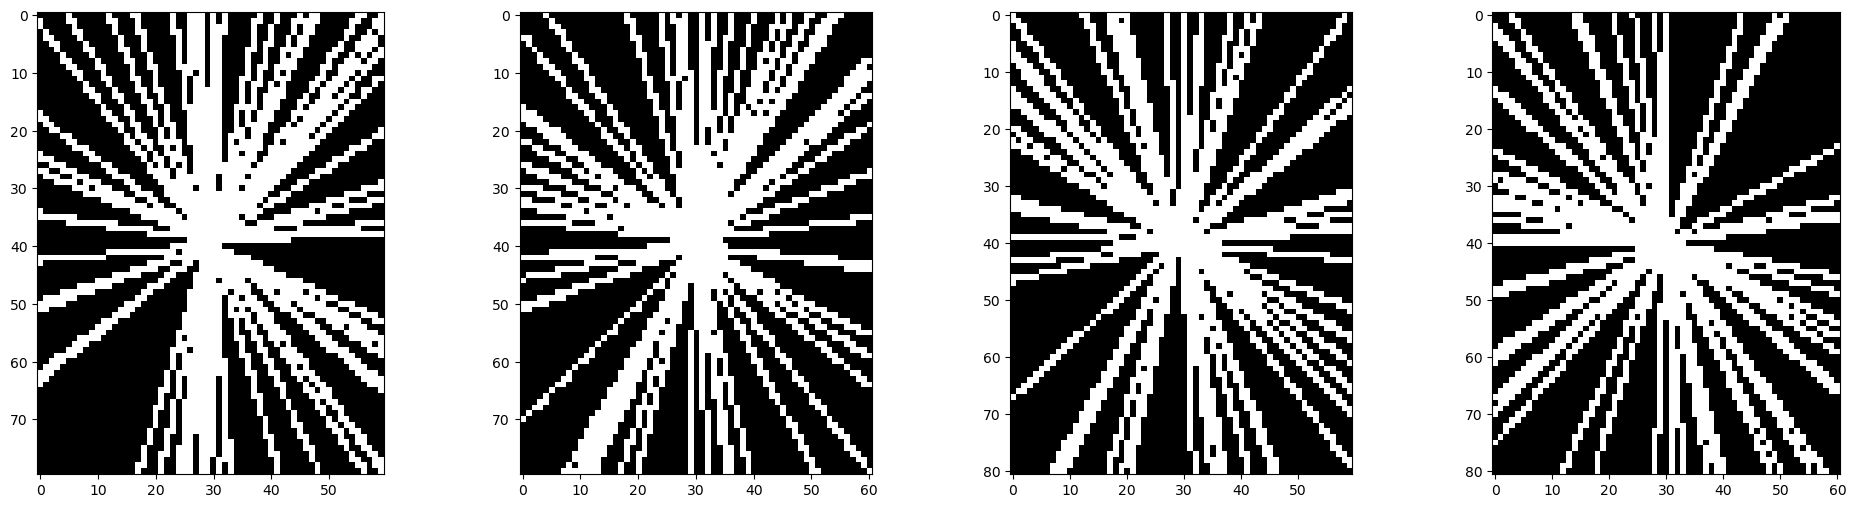
\includegraphics[width=\textwidth]{mask}}
\caption{Radially retained sampling ---
         sampling on a Cartesian grid along rays emanating from the origin}
\label{radialines}
\end{figure}




\newlength{\vertsep}
\setlength{\vertsep}{.0in}
\newlength{\imsize}
\setlength{\imsize}{.34\textwidth}
\newlength{\imsizes}
\setlength{\imsizes}{.49\textwidth}


\begin{figure}
\begin{centering}

\parbox{\imsize}{\includegraphics[width=\imsize]{../brainsout/r3j_error}}
\parbox{\imsize}{\includegraphics[width=\imsize]{../brainsout/r3j_jackknife}}

\vspace{\vertsep}

\parbox{\imsize}{\includegraphics[width=\imsize]{../brainsout/r3_original}}
\parbox{\imsize}{\includegraphics[width=\imsize]{../brainsout/r3_recon}}

\vspace{\vertsep}

\parbox{\imsize}{\includegraphics[width=\imsize]{../brainsout/r3_error}}
\parbox{\imsize}{\includegraphics[width=\imsize]{../brainsout/r3_bootstrap}}

\end{centering}
\caption{Radially retained sampling --- lower slice}
\label{bigradial}
\end{figure}


\begin{figure}
\begin{centering}

\parbox{\imsize}{\includegraphics[width=\imsize]{../brainsout/r10j_error}}
\parbox{\imsize}{\includegraphics[width=\imsize]{../brainsout/r10j_jackknife}}

\vspace{\vertsep}

\parbox{\imsize}{\includegraphics[width=\imsize]{../brainsout/r10_original}}
\parbox{\imsize}{\includegraphics[width=\imsize]{../brainsout/r10_recon}}

\vspace{\vertsep}

\parbox{\imsize}{\includegraphics[width=\imsize]{../brainsout/r10_error}}
\parbox{\imsize}{\includegraphics[width=\imsize]{../brainsout/r10_bootstrap}}

\end{centering}
\caption{Radially retained sampling --- upper slice}
\label{afterbigradial}
\end{figure}


\begin{figure}
\begin{centering}

\parbox{\imsize}{\includegraphics[width=\imsize]{../brainsout/h3j_error}}
\parbox{\imsize}{\includegraphics[width=\imsize]{../brainsout/h3j_jackknife}}

\vspace{\vertsep}

\parbox{\imsize}{\includegraphics[width=\imsize]{../brainsout/h3_original}}
\parbox{\imsize}{\includegraphics[width=\imsize]{../brainsout/h3_recon}}

\vspace{\vertsep}

\parbox{\imsize}{\includegraphics[width=\imsize]{../brainsout/h3_error}}
\parbox{\imsize}{\includegraphics[width=\imsize]{../brainsout/h3_bootstrap}}

\end{centering}
\caption{Horizontally retained sampling --- lower slice}
\end{figure}


\begin{figure}
\begin{centering}

\parbox{\imsize}{\includegraphics[width=\imsize]{../brainsout/h10j_error}}
\parbox{\imsize}{\includegraphics[width=\imsize]{../brainsout/h10j_jackknife}}

\vspace{\vertsep}

\parbox{\imsize}{\includegraphics[width=\imsize]{../brainsout/h10_original}}
\parbox{\imsize}{\includegraphics[width=\imsize]{../brainsout/h10_recon}}

\vspace{\vertsep}

\parbox{\imsize}{\includegraphics[width=\imsize]{../brainsout/h10_error}}
\parbox{\imsize}{\includegraphics[width=\imsize]{../brainsout/h10_bootstrap}}

\end{centering}
\caption{Horizontally retained sampling --- upper slice}
\label{bighorizontal}
\end{figure}


\begin{figure}
\begin{centering}

\parbox{\imsizes}{\includegraphics[width=\imsizes]{../brainsout/r3_original}}
\hfill
\parbox{\imsizes}{\includegraphics[width=\imsizes]{../brainsout/r3_recon}}

\vspace{\vertsep}

\parbox{\imsizes}{\includegraphics[width=\imsizes]{../brainsout/r3_corrected}}
\hfill
\parbox{\imsizes}{\includegraphics[width=\imsizes]{../brainsout/r3_overlaid}}

\end{centering}
\caption{Radially retained sampling --- lower slice (a)}
\label{first_viz}
\end{figure}


\begin{figure}
\begin{centering}

\parbox{\imsizes}{\includegraphics[width=\imsizes]{../brainsout/r3_saturated}}
\hfill
\parbox{\imsizes}{\includegraphics[width=\imsizes]
       {../brainsout/r3_interpolated}}

\vspace{\vertsep}

\parbox{\imsizes}{\includegraphics[width=\imsizes]{../brainsout/r3_error}}
\hfill
\parbox{\imsizes}{\includegraphics[width=\imsizes]{../brainsout/r3_bootstrap}}

\end{centering}
\caption{Radially retained sampling --- lower slice (b)}
\end{figure}


\begin{figure}
\begin{centering}

\parbox{\imsizes}{\includegraphics[width=\imsizes]{../brainsout/r10_original}}
\hfill
\parbox{\imsizes}{\includegraphics[width=\imsizes]{../brainsout/r10_recon}}

\vspace{\vertsep}

\parbox{\imsizes}{\includegraphics[width=\imsizes]{../brainsout/r10_corrected}}
\hfill
\parbox{\imsizes}{\includegraphics[width=\imsizes]{../brainsout/r10_overlaid}}

\end{centering}
\caption{Radially retained sampling --- upper slice (a)}
\end{figure}


\begin{figure}
\begin{centering}

\parbox{\imsizes}{\includegraphics[width=\imsizes]{../brainsout/r10_saturated}}
\hfill
\parbox{\imsizes}{\includegraphics[width=\imsizes]
       {../brainsout/r10_interpolated}}

\vspace{\vertsep}

\parbox{\imsizes}{\includegraphics[width=\imsizes]{../brainsout/r10_error}}
\hfill
\parbox{\imsizes}{\includegraphics[width=\imsizes]{../brainsout/r10_bootstrap}}

\end{centering}
\caption{Radially retained sampling --- upper slice (b)}
\end{figure}


\begin{figure}
\begin{centering}

\parbox{\imsizes}{\includegraphics[width=\imsizes]{../brainsout/h3_original}}
\hfill
\parbox{\imsizes}{\includegraphics[width=\imsizes]{../brainsout/h3_recon}}

\vspace{\vertsep}

\parbox{\imsizes}{\includegraphics[width=\imsizes]{../brainsout/h3_corrected}}
\hfill
\parbox{\imsizes}{\includegraphics[width=\imsizes]{../brainsout/h3_overlaid}}

\end{centering}
\caption{Horizontally retained sampling --- lower slice (a)}
\end{figure}


\begin{figure}
\begin{centering}

\parbox{\imsizes}{\includegraphics[width=\imsizes]{../brainsout/h3_saturated}}
\hfill
\parbox{\imsizes}{\includegraphics[width=\imsizes]
       {../brainsout/h3_interpolated}}

\vspace{\vertsep}

\parbox{\imsizes}{\includegraphics[width=\imsizes]{../brainsout/h3_error}}
\hfill
\parbox{\imsizes}{\includegraphics[width=\imsizes]{../brainsout/h3_bootstrap}}

\end{centering}
\caption{Horizontally retained sampling --- lower slice (b)}
\end{figure}


\begin{figure}
\begin{centering}

\parbox{\imsizes}{\includegraphics[width=\imsizes]{../brainsout/h10_original}}
\hfill
\parbox{\imsizes}{\includegraphics[width=\imsizes]{../brainsout/h10_recon}}

\vspace{\vertsep}

\parbox{\imsizes}{\includegraphics[width=\imsizes]{../brainsout/h10_corrected}}
\hfill
\parbox{\imsizes}{\includegraphics[width=\imsizes]{../brainsout/h10_overlaid}}

\end{centering}
\caption{Horizontally retained sampling --- upper slice (a)}
\end{figure}


\begin{figure}
\begin{centering}

\parbox{\imsizes}{\includegraphics[width=\imsizes]{../brainsout/h10_saturated}}
\hfill
\parbox{\imsizes}{\includegraphics[width=\imsizes]
       {../brainsout/h10_interpolated}}

\vspace{\vertsep}

\parbox{\imsizes}{\includegraphics[width=\imsizes]{../brainsout/h10_error}}
\hfill
\parbox{\imsizes}{\includegraphics[width=\imsizes]{../brainsout/h10_bootstrap}}

\end{centering}
\caption{Horizontally retained sampling --- upper slice (b)}
\label{last_viz}
\end{figure}


\begin{figure}
\begin{centering}

\parbox{\imsizes}{\includegraphics[width=\imsizes]{../brainsout/r10_bootstrap}}
\hfill
\parbox{\imsizes}{\includegraphics[width=\imsizes]{../brainsout/r10_blurred}}

\vspace{\vertsep}

\parbox{\imsizes}{\includegraphics[width=\imsizes]{../brainsout/r3_bootstrap}}
\hfill
\parbox{\imsizes}{\includegraphics[width=\imsizes]{../brainsout/r3_blurred}}

\end{centering}
\caption{Radially retained sampling
--- upper plots display the upper slice; lower plots display the lower}
\label{blurredr}
\end{figure}


\begin{figure}
\begin{centering}

\parbox{\imsizes}{\includegraphics[width=\imsizes]{../brainsout/h10_bootstrap}}
\hfill
\parbox{\imsizes}{\includegraphics[width=\imsizes]{../brainsout/h10_blurred}}

\vspace{\vertsep}

\parbox{\imsizes}{\includegraphics[width=\imsizes]{../brainsout/h3_bootstrap}}
\hfill
\parbox{\imsizes}{\includegraphics[width=\imsizes]{../brainsout/h3_blurred}}

\end{centering}
\caption{Horizontally retained sampling
--- upper plots display the upper slice; lower plots display the lower}
\label{blurredh}
\end{figure}



\begin{table}
\caption{Square roots of the sums of the squares of the error estimates}
\label{blurring}
\begin{centering}

\vspace{.125in}

\begin{tabular}{llll}
\hline
    Sampling & Slice & Bootstrap & Blurred Bootstrap \\\hline
horizontally & lower &      12.9 &              6.25 \\
horizontally & upper &      13.8 &              7.34 \\
    radially & lower &      17.5 &              10.5 \\
    radially & upper &      18.0 &              11.6 \\\hline
\end{tabular}

\end{centering}
\end{table}



\begin{table}

\vspace{.125in}

\caption{Square roots of the sums of the squares of the error estimates
for the lower slice blurred against a Gaussian convolutional kernel
of the specified standard deviation (the standard deviation is in pixels),
for sampling retained horizontally or radially}
\label{blurs3}
\begin{centering}

\vspace{.125in}

\begin{tabular}{lll}
\hline Std.\ Dev. & Horizontally & Radially \\\hline
       0.0 &         12.9 &     17.5 \\
       0.5 &         9.94 &     14.6 \\
       1.0 &         6.25 &     10.5 \\
       1.5 &         4.38 &     8.06 \\
       2.0 &         3.03 &     6.34 \\
       2.5 &         2.04 &     5.06 \\
       3.0 &         1.33 &     4.09 \\
       3.5 &         .847 &     3.34 \\
       4.0 &         .535 &     2.75 \\\hline
\end{tabular}

\end{centering}
\end{table}



\begin{table}

\vspace{.125in}

\caption{Square roots of the sums of the squares of the error estimates
for the upper slice blurred against a Gaussian convolutional kernel
of the specified standard deviation (the standard deviation is in pixels),
for sampling retained horizontally or radially}
\label{blurs10}
\begin{centering}

\vspace{.125in}

\begin{tabular}{lll}
\hline Std.\ Dev. & Horizontally & Radially \\\hline
       0.0 &         13.8 &     18.0 \\
       0.5 &         10.9 &     15.3 \\
       1.0 &         7.34 &     11.6 \\
       1.5 &         5.35 &     9.50 \\
       2.0 &         3.82 &     7.97 \\
       2.5 &         2.63 &     6.79 \\
       3.0 &         1.75 &     5.87 \\
       3.5 &         1.14 &     5.13 \\
       4.0 &         .745 &     4.54 \\\hline
\end{tabular}

\end{centering}
\end{table}




%% -- Bibliography -------------------------------------------------------------
%% - References need to be provided in a .bib BibTeX database.
%% - All references should be made with \cite, \citet, \citep, \citealp etc.
%%   (and never hard-coded). See the FAQ for details.
%% - JSS-specific markup (\proglang, \pkg, \code) should be used in the .bib.
%% - Titles in the .bib should be in title case.
%% - DOIs should be included where available.

\clearpage
\bibliography{fbooja}




%% -- Appendix (if any) --------------------------------------------------------
%% - After the bibliography with page break.
%% - With proper section titles and _not_ just "Appendix".

\newpage

\begin{appendix}

\section{Supplementary jackknives and bootstraps}
\label{suppfigs}

This appendix supplements Figures~\ref{bigradial}--\ref{bighorizontal}
of Section~\ref{results} with analogous figures
for twenty cross-sectional slices through the head of the patient
(Figures~\ref{bigradial}--\ref{bighorizontal} are for slices 3 and 10).


\begin{figure}
\begin{centering}

\parbox{\imsize}{\includegraphics[width=\imsize]{../brainsout/r1j_error}}
\parbox{\imsize}{\includegraphics[width=\imsize]{../brainsout/r1j_jackknife}}

\vspace{\vertsep}

\parbox{\imsize}{\includegraphics[width=\imsize]{../brainsout/r1_original}}
\parbox{\imsize}{\includegraphics[width=\imsize]{../brainsout/r1_recon}}

\vspace{\vertsep}

\parbox{\imsize}{\includegraphics[width=\imsize]{../brainsout/r1_error}}
\parbox{\imsize}{\includegraphics[width=\imsize]{../brainsout/r1_bootstrap}}

\end{centering}
\caption{Radially retained sampling --- slice 1}
\end{figure}


\begin{figure}
\begin{centering}

\parbox{\imsize}{\includegraphics[width=\imsize]{../brainsout/r2j_error}}
\parbox{\imsize}{\includegraphics[width=\imsize]{../brainsout/r2j_jackknife}}

\vspace{\vertsep}

\parbox{\imsize}{\includegraphics[width=\imsize]{../brainsout/r2_original}}
\parbox{\imsize}{\includegraphics[width=\imsize]{../brainsout/r2_recon}}

\vspace{\vertsep}

\parbox{\imsize}{\includegraphics[width=\imsize]{../brainsout/r2_error}}
\parbox{\imsize}{\includegraphics[width=\imsize]{../brainsout/r2_bootstrap}}

\end{centering}
\caption{Radially retained sampling --- slice 2}
\end{figure}


\begin{figure}
\begin{centering}

\parbox{\imsize}{\includegraphics[width=\imsize]{../brainsout/r3j_error}}
\parbox{\imsize}{\includegraphics[width=\imsize]{../brainsout/r3j_jackknife}}

\vspace{\vertsep}

\parbox{\imsize}{\includegraphics[width=\imsize]{../brainsout/r3_original}}
\parbox{\imsize}{\includegraphics[width=\imsize]{../brainsout/r3_recon}}

\vspace{\vertsep}

\parbox{\imsize}{\includegraphics[width=\imsize]{../brainsout/r3_error}}
\parbox{\imsize}{\includegraphics[width=\imsize]{../brainsout/r3_bootstrap}}

\end{centering}
\caption{Radially retained sampling --- slice 3}
\end{figure}


\begin{figure}
\begin{centering}

\parbox{\imsize}{\includegraphics[width=\imsize]{../brainsout/r4j_error}}
\parbox{\imsize}{\includegraphics[width=\imsize]{../brainsout/r4j_jackknife}}

\vspace{\vertsep}

\parbox{\imsize}{\includegraphics[width=\imsize]{../brainsout/r4_original}}
\parbox{\imsize}{\includegraphics[width=\imsize]{../brainsout/r4_recon}}

\vspace{\vertsep}

\parbox{\imsize}{\includegraphics[width=\imsize]{../brainsout/r4_error}}
\parbox{\imsize}{\includegraphics[width=\imsize]{../brainsout/r4_bootstrap}}

\end{centering}
\caption{Radially retained sampling --- slice 4}
\end{figure}


\begin{figure}
\begin{centering}

\parbox{\imsize}{\includegraphics[width=\imsize]{../brainsout/r5j_error}}
\parbox{\imsize}{\includegraphics[width=\imsize]{../brainsout/r5j_jackknife}}

\vspace{\vertsep}

\parbox{\imsize}{\includegraphics[width=\imsize]{../brainsout/r5_original}}
\parbox{\imsize}{\includegraphics[width=\imsize]{../brainsout/r5_recon}}

\vspace{\vertsep}

\parbox{\imsize}{\includegraphics[width=\imsize]{../brainsout/r5_error}}
\parbox{\imsize}{\includegraphics[width=\imsize]{../brainsout/r5_bootstrap}}

\end{centering}
\caption{Radially retained sampling --- slice 5}
\end{figure}


\begin{figure}
\begin{centering}

\parbox{\imsize}{\includegraphics[width=\imsize]{../brainsout/r6j_error}}
\parbox{\imsize}{\includegraphics[width=\imsize]{../brainsout/r6j_jackknife}}

\vspace{\vertsep}

\parbox{\imsize}{\includegraphics[width=\imsize]{../brainsout/r6_original}}
\parbox{\imsize}{\includegraphics[width=\imsize]{../brainsout/r6_recon}}

\vspace{\vertsep}

\parbox{\imsize}{\includegraphics[width=\imsize]{../brainsout/r6_error}}
\parbox{\imsize}{\includegraphics[width=\imsize]{../brainsout/r6_bootstrap}}

\end{centering}
\caption{Radially retained sampling --- slice 6}
\end{figure}


\begin{figure}
\begin{centering}

\parbox{\imsize}{\includegraphics[width=\imsize]{../brainsout/r7j_error}}
\parbox{\imsize}{\includegraphics[width=\imsize]{../brainsout/r7j_jackknife}}

\vspace{\vertsep}

\parbox{\imsize}{\includegraphics[width=\imsize]{../brainsout/r7_original}}
\parbox{\imsize}{\includegraphics[width=\imsize]{../brainsout/r7_recon}}

\vspace{\vertsep}

\parbox{\imsize}{\includegraphics[width=\imsize]{../brainsout/r7_error}}
\parbox{\imsize}{\includegraphics[width=\imsize]{../brainsout/r7_bootstrap}}

\end{centering}
\caption{Radially retained sampling --- slice 7}
\end{figure}


\begin{figure}
\begin{centering}

\parbox{\imsize}{\includegraphics[width=\imsize]{../brainsout/r8j_error}}
\parbox{\imsize}{\includegraphics[width=\imsize]{../brainsout/r8j_jackknife}}

\vspace{\vertsep}

\parbox{\imsize}{\includegraphics[width=\imsize]{../brainsout/r8_original}}
\parbox{\imsize}{\includegraphics[width=\imsize]{../brainsout/r8_recon}}

\vspace{\vertsep}

\parbox{\imsize}{\includegraphics[width=\imsize]{../brainsout/r8_error}}
\parbox{\imsize}{\includegraphics[width=\imsize]{../brainsout/r8_bootstrap}}

\end{centering}
\caption{Radially retained sampling --- slice 8}
\end{figure}


\begin{figure}
\begin{centering}

\parbox{\imsize}{\includegraphics[width=\imsize]{../brainsout/r9j_error}}
\parbox{\imsize}{\includegraphics[width=\imsize]{../brainsout/r9j_jackknife}}

\vspace{\vertsep}

\parbox{\imsize}{\includegraphics[width=\imsize]{../brainsout/r9_original}}
\parbox{\imsize}{\includegraphics[width=\imsize]{../brainsout/r9_recon}}

\vspace{\vertsep}

\parbox{\imsize}{\includegraphics[width=\imsize]{../brainsout/r9_error}}
\parbox{\imsize}{\includegraphics[width=\imsize]{../brainsout/r9_bootstrap}}

\end{centering}
\caption{Radially retained sampling --- slice 9}
\end{figure}


\begin{figure}
\begin{centering}

\parbox{\imsize}{\includegraphics[width=\imsize]{../brainsout/r10j_error}}
\parbox{\imsize}{\includegraphics[width=\imsize]{../brainsout/r10j_jackknife}}

\vspace{\vertsep}

\parbox{\imsize}{\includegraphics[width=\imsize]{../brainsout/r10_original}}
\parbox{\imsize}{\includegraphics[width=\imsize]{../brainsout/r10_recon}}

\vspace{\vertsep}

\parbox{\imsize}{\includegraphics[width=\imsize]{../brainsout/r10_error}}
\parbox{\imsize}{\includegraphics[width=\imsize]{../brainsout/r10_bootstrap}}

\end{centering}
\caption{Radially retained sampling --- slice 10}
\end{figure}


\begin{figure}
\begin{centering}

\parbox{\imsize}{\includegraphics[width=\imsize]{../brainsout/r11j_error}}
\parbox{\imsize}{\includegraphics[width=\imsize]{../brainsout/r11j_jackknife}}

\vspace{\vertsep}

\parbox{\imsize}{\includegraphics[width=\imsize]{../brainsout/r11_original}}
\parbox{\imsize}{\includegraphics[width=\imsize]{../brainsout/r11_recon}}

\vspace{\vertsep}

\parbox{\imsize}{\includegraphics[width=\imsize]{../brainsout/r11_error}}
\parbox{\imsize}{\includegraphics[width=\imsize]{../brainsout/r11_bootstrap}}

\end{centering}
\caption{Radially retained sampling --- slice 11}
\end{figure}


\begin{figure}
\begin{centering}

\parbox{\imsize}{\includegraphics[width=\imsize]{../brainsout/r12j_error}}
\parbox{\imsize}{\includegraphics[width=\imsize]{../brainsout/r12j_jackknife}}

\vspace{\vertsep}

\parbox{\imsize}{\includegraphics[width=\imsize]{../brainsout/r12_original}}
\parbox{\imsize}{\includegraphics[width=\imsize]{../brainsout/r12_recon}}

\vspace{\vertsep}

\parbox{\imsize}{\includegraphics[width=\imsize]{../brainsout/r12_error}}
\parbox{\imsize}{\includegraphics[width=\imsize]{../brainsout/r12_bootstrap}}

\end{centering}
\caption{Radially retained sampling --- slice 12}
\end{figure}


\begin{figure}
\begin{centering}

\parbox{\imsize}{\includegraphics[width=\imsize]{../brainsout/r13j_error}}
\parbox{\imsize}{\includegraphics[width=\imsize]{../brainsout/r13j_jackknife}}

\vspace{\vertsep}

\parbox{\imsize}{\includegraphics[width=\imsize]{../brainsout/r13_original}}
\parbox{\imsize}{\includegraphics[width=\imsize]{../brainsout/r13_recon}}

\vspace{\vertsep}

\parbox{\imsize}{\includegraphics[width=\imsize]{../brainsout/r13_error}}
\parbox{\imsize}{\includegraphics[width=\imsize]{../brainsout/r13_bootstrap}}

\end{centering}
\caption{Radially retained sampling --- slice 13}
\end{figure}


\begin{figure}
\begin{centering}

\parbox{\imsize}{\includegraphics[width=\imsize]{../brainsout/r14j_error}}
\parbox{\imsize}{\includegraphics[width=\imsize]{../brainsout/r14j_jackknife}}

\vspace{\vertsep}

\parbox{\imsize}{\includegraphics[width=\imsize]{../brainsout/r14_original}}
\parbox{\imsize}{\includegraphics[width=\imsize]{../brainsout/r14_recon}}

\vspace{\vertsep}

\parbox{\imsize}{\includegraphics[width=\imsize]{../brainsout/r14_error}}
\parbox{\imsize}{\includegraphics[width=\imsize]{../brainsout/r14_bootstrap}}

\end{centering}
\caption{Radially retained sampling --- slice 14}
\end{figure}


\begin{figure}
\begin{centering}

\parbox{\imsize}{\includegraphics[width=\imsize]{../brainsout/r15j_error}}
\parbox{\imsize}{\includegraphics[width=\imsize]{../brainsout/r15j_jackknife}}

\vspace{\vertsep}

\parbox{\imsize}{\includegraphics[width=\imsize]{../brainsout/r15_original}}
\parbox{\imsize}{\includegraphics[width=\imsize]{../brainsout/r15_recon}}

\vspace{\vertsep}

\parbox{\imsize}{\includegraphics[width=\imsize]{../brainsout/r15_error}}
\parbox{\imsize}{\includegraphics[width=\imsize]{../brainsout/r15_bootstrap}}

\end{centering}
\caption{Radially retained sampling --- slice 15}
\end{figure}


\begin{figure}
\begin{centering}

\parbox{\imsize}{\includegraphics[width=\imsize]{../brainsout/r16j_error}}
\parbox{\imsize}{\includegraphics[width=\imsize]{../brainsout/r16j_jackknife}}

\vspace{\vertsep}

\parbox{\imsize}{\includegraphics[width=\imsize]{../brainsout/r16_original}}
\parbox{\imsize}{\includegraphics[width=\imsize]{../brainsout/r16_recon}}

\vspace{\vertsep}

\parbox{\imsize}{\includegraphics[width=\imsize]{../brainsout/r16_error}}
\parbox{\imsize}{\includegraphics[width=\imsize]{../brainsout/r16_bootstrap}}

\end{centering}
\caption{Radially retained sampling --- slice 16}
\end{figure}


\begin{figure}
\begin{centering}

\parbox{\imsize}{\includegraphics[width=\imsize]{../brainsout/r17j_error}}
\parbox{\imsize}{\includegraphics[width=\imsize]{../brainsout/r17j_jackknife}}

\vspace{\vertsep}

\parbox{\imsize}{\includegraphics[width=\imsize]{../brainsout/r17_original}}
\parbox{\imsize}{\includegraphics[width=\imsize]{../brainsout/r17_recon}}

\vspace{\vertsep}

\parbox{\imsize}{\includegraphics[width=\imsize]{../brainsout/r17_error}}
\parbox{\imsize}{\includegraphics[width=\imsize]{../brainsout/r17_bootstrap}}

\end{centering}
\caption{Radially retained sampling --- slice 17}
\end{figure}


\begin{figure}
\begin{centering}

\parbox{\imsize}{\includegraphics[width=\imsize]{../brainsout/r18j_error}}
\parbox{\imsize}{\includegraphics[width=\imsize]{../brainsout/r18j_jackknife}}

\vspace{\vertsep}

\parbox{\imsize}{\includegraphics[width=\imsize]{../brainsout/r18_original}}
\parbox{\imsize}{\includegraphics[width=\imsize]{../brainsout/r18_recon}}

\vspace{\vertsep}

\parbox{\imsize}{\includegraphics[width=\imsize]{../brainsout/r18_error}}
\parbox{\imsize}{\includegraphics[width=\imsize]{../brainsout/r18_bootstrap}}

\end{centering}
\caption{Radially retained sampling --- slice 18}
\end{figure}


\begin{figure}
\begin{centering}

\parbox{\imsize}{\includegraphics[width=\imsize]{../brainsout/r19j_error}}
\parbox{\imsize}{\includegraphics[width=\imsize]{../brainsout/r19j_jackknife}}

\vspace{\vertsep}

\parbox{\imsize}{\includegraphics[width=\imsize]{../brainsout/r19_original}}
\parbox{\imsize}{\includegraphics[width=\imsize]{../brainsout/r19_recon}}

\vspace{\vertsep}

\parbox{\imsize}{\includegraphics[width=\imsize]{../brainsout/r19_error}}
\parbox{\imsize}{\includegraphics[width=\imsize]{../brainsout/r19_bootstrap}}

\end{centering}
\caption{Radially retained sampling --- slice 19}
\end{figure}


\begin{figure}
\begin{centering}

\parbox{\imsize}{\includegraphics[width=\imsize]{../brainsout/r20j_error}}
\parbox{\imsize}{\includegraphics[width=\imsize]{../brainsout/r20j_jackknife}}

\vspace{\vertsep}

\parbox{\imsize}{\includegraphics[width=\imsize]{../brainsout/r20_original}}
\parbox{\imsize}{\includegraphics[width=\imsize]{../brainsout/r20_recon}}

\vspace{\vertsep}

\parbox{\imsize}{\includegraphics[width=\imsize]{../brainsout/r20_error}}
\parbox{\imsize}{\includegraphics[width=\imsize]{../brainsout/r20_bootstrap}}

\end{centering}
\caption{Radially retained sampling --- slice 20}
\end{figure}


\begin{figure}
\begin{centering}

\parbox{\imsize}{\includegraphics[width=\imsize]{../brainsout/h1j_error}}
\parbox{\imsize}{\includegraphics[width=\imsize]{../brainsout/h1j_jackknife}}

\vspace{\vertsep}

\parbox{\imsize}{\includegraphics[width=\imsize]{../brainsout/h1_original}}
\parbox{\imsize}{\includegraphics[width=\imsize]{../brainsout/h1_recon}}

\vspace{\vertsep}

\parbox{\imsize}{\includegraphics[width=\imsize]{../brainsout/h1_error}}
\parbox{\imsize}{\includegraphics[width=\imsize]{../brainsout/h1_bootstrap}}

\end{centering}
\caption{Horizontally retained sampling --- slice 1}
\end{figure}


\begin{figure}
\begin{centering}

\parbox{\imsize}{\includegraphics[width=\imsize]{../brainsout/h2j_error}}
\parbox{\imsize}{\includegraphics[width=\imsize]{../brainsout/h2j_jackknife}}

\vspace{\vertsep}

\parbox{\imsize}{\includegraphics[width=\imsize]{../brainsout/h2_original}}
\parbox{\imsize}{\includegraphics[width=\imsize]{../brainsout/h2_recon}}

\vspace{\vertsep}

\parbox{\imsize}{\includegraphics[width=\imsize]{../brainsout/h2_error}}
\parbox{\imsize}{\includegraphics[width=\imsize]{../brainsout/h2_bootstrap}}

\end{centering}
\caption{Horizontally retained sampling --- slice 2}
\end{figure}


\begin{figure}
\begin{centering}

\parbox{\imsize}{\includegraphics[width=\imsize]{../brainsout/h3j_error}}
\parbox{\imsize}{\includegraphics[width=\imsize]{../brainsout/h3j_jackknife}}

\vspace{\vertsep}

\parbox{\imsize}{\includegraphics[width=\imsize]{../brainsout/h3_original}}
\parbox{\imsize}{\includegraphics[width=\imsize]{../brainsout/h3_recon}}

\vspace{\vertsep}

\parbox{\imsize}{\includegraphics[width=\imsize]{../brainsout/h3_error}}
\parbox{\imsize}{\includegraphics[width=\imsize]{../brainsout/h3_bootstrap}}

\end{centering}
\caption{Horizontally retained sampling --- slice 3}
\end{figure}


\begin{figure}
\begin{centering}

\parbox{\imsize}{\includegraphics[width=\imsize]{../brainsout/h4j_error}}
\parbox{\imsize}{\includegraphics[width=\imsize]{../brainsout/h4j_jackknife}}

\vspace{\vertsep}

\parbox{\imsize}{\includegraphics[width=\imsize]{../brainsout/h4_original}}
\parbox{\imsize}{\includegraphics[width=\imsize]{../brainsout/h4_recon}}

\vspace{\vertsep}

\parbox{\imsize}{\includegraphics[width=\imsize]{../brainsout/h4_error}}
\parbox{\imsize}{\includegraphics[width=\imsize]{../brainsout/h4_bootstrap}}

\end{centering}
\caption{Horizontally retained sampling --- slice 4}
\end{figure}


\begin{figure}
\begin{centering}

\parbox{\imsize}{\includegraphics[width=\imsize]{../brainsout/h5j_error}}
\parbox{\imsize}{\includegraphics[width=\imsize]{../brainsout/h5j_jackknife}}

\vspace{\vertsep}

\parbox{\imsize}{\includegraphics[width=\imsize]{../brainsout/h5_original}}
\parbox{\imsize}{\includegraphics[width=\imsize]{../brainsout/h5_recon}}

\vspace{\vertsep}

\parbox{\imsize}{\includegraphics[width=\imsize]{../brainsout/h5_error}}
\parbox{\imsize}{\includegraphics[width=\imsize]{../brainsout/h5_bootstrap}}

\end{centering}
\caption{Horizontally retained sampling --- slice 5}
\end{figure}


\begin{figure}
\begin{centering}

\parbox{\imsize}{\includegraphics[width=\imsize]{../brainsout/h6j_error}}
\parbox{\imsize}{\includegraphics[width=\imsize]{../brainsout/h6j_jackknife}}

\vspace{\vertsep}

\parbox{\imsize}{\includegraphics[width=\imsize]{../brainsout/h6_original}}
\parbox{\imsize}{\includegraphics[width=\imsize]{../brainsout/h6_recon}}

\vspace{\vertsep}

\parbox{\imsize}{\includegraphics[width=\imsize]{../brainsout/h6_error}}
\parbox{\imsize}{\includegraphics[width=\imsize]{../brainsout/h6_bootstrap}}

\end{centering}
\caption{Horizontally retained sampling --- slice 6}
\end{figure}


\begin{figure}
\begin{centering}

\parbox{\imsize}{\includegraphics[width=\imsize]{../brainsout/h7j_error}}
\parbox{\imsize}{\includegraphics[width=\imsize]{../brainsout/h7j_jackknife}}

\vspace{\vertsep}

\parbox{\imsize}{\includegraphics[width=\imsize]{../brainsout/h7_original}}
\parbox{\imsize}{\includegraphics[width=\imsize]{../brainsout/h7_recon}}

\vspace{\vertsep}

\parbox{\imsize}{\includegraphics[width=\imsize]{../brainsout/h7_error}}
\parbox{\imsize}{\includegraphics[width=\imsize]{../brainsout/h7_bootstrap}}

\end{centering}
\caption{Horizontally retained sampling --- slice 7}
\end{figure}


\begin{figure}
\begin{centering}

\parbox{\imsize}{\includegraphics[width=\imsize]{../brainsout/h8j_error}}
\parbox{\imsize}{\includegraphics[width=\imsize]{../brainsout/h8j_jackknife}}

\vspace{\vertsep}

\parbox{\imsize}{\includegraphics[width=\imsize]{../brainsout/h8_original}}
\parbox{\imsize}{\includegraphics[width=\imsize]{../brainsout/h8_recon}}

\vspace{\vertsep}

\parbox{\imsize}{\includegraphics[width=\imsize]{../brainsout/h8_error}}
\parbox{\imsize}{\includegraphics[width=\imsize]{../brainsout/h8_bootstrap}}

\end{centering}
\caption{Horizontally retained sampling --- slice 8}
\end{figure}


\begin{figure}
\begin{centering}

\parbox{\imsize}{\includegraphics[width=\imsize]{../brainsout/h9j_error}}
\parbox{\imsize}{\includegraphics[width=\imsize]{../brainsout/h9j_jackknife}}

\vspace{\vertsep}

\parbox{\imsize}{\includegraphics[width=\imsize]{../brainsout/h9_original}}
\parbox{\imsize}{\includegraphics[width=\imsize]{../brainsout/h9_recon}}

\vspace{\vertsep}

\parbox{\imsize}{\includegraphics[width=\imsize]{../brainsout/h9_error}}
\parbox{\imsize}{\includegraphics[width=\imsize]{../brainsout/h9_bootstrap}}

\end{centering}
\caption{Horizontally retained sampling --- slice 9}
\end{figure}


\begin{figure}
\begin{centering}

\parbox{\imsize}{\includegraphics[width=\imsize]{../brainsout/h10j_error}}
\parbox{\imsize}{\includegraphics[width=\imsize]{../brainsout/h10j_jackknife}}

\vspace{\vertsep}

\parbox{\imsize}{\includegraphics[width=\imsize]{../brainsout/h10_original}}
\parbox{\imsize}{\includegraphics[width=\imsize]{../brainsout/h10_recon}}

\vspace{\vertsep}

\parbox{\imsize}{\includegraphics[width=\imsize]{../brainsout/h10_error}}
\parbox{\imsize}{\includegraphics[width=\imsize]{../brainsout/h10_bootstrap}}

\end{centering}
\caption{Horizontally retained sampling --- slice 10}
\end{figure}


\begin{figure}
\begin{centering}

\parbox{\imsize}{\includegraphics[width=\imsize]{../brainsout/h11j_error}}
\parbox{\imsize}{\includegraphics[width=\imsize]{../brainsout/h11j_jackknife}}

\vspace{\vertsep}

\parbox{\imsize}{\includegraphics[width=\imsize]{../brainsout/h11_original}}
\parbox{\imsize}{\includegraphics[width=\imsize]{../brainsout/h11_recon}}

\vspace{\vertsep}

\parbox{\imsize}{\includegraphics[width=\imsize]{../brainsout/h11_error}}
\parbox{\imsize}{\includegraphics[width=\imsize]{../brainsout/h11_bootstrap}}

\end{centering}
\caption{Horizontally retained sampling --- slice 11}
\end{figure}


\begin{figure}
\begin{centering}

\parbox{\imsize}{\includegraphics[width=\imsize]{../brainsout/h12j_error}}
\parbox{\imsize}{\includegraphics[width=\imsize]{../brainsout/h12j_jackknife}}

\vspace{\vertsep}

\parbox{\imsize}{\includegraphics[width=\imsize]{../brainsout/h12_original}}
\parbox{\imsize}{\includegraphics[width=\imsize]{../brainsout/h12_recon}}

\vspace{\vertsep}

\parbox{\imsize}{\includegraphics[width=\imsize]{../brainsout/h12_error}}
\parbox{\imsize}{\includegraphics[width=\imsize]{../brainsout/h12_bootstrap}}

\end{centering}
\caption{Horizontally retained sampling --- slice 12}
\end{figure}


\begin{figure}
\begin{centering}

\parbox{\imsize}{\includegraphics[width=\imsize]{../brainsout/h13j_error}}
\parbox{\imsize}{\includegraphics[width=\imsize]{../brainsout/h13j_jackknife}}

\vspace{\vertsep}

\parbox{\imsize}{\includegraphics[width=\imsize]{../brainsout/h13_original}}
\parbox{\imsize}{\includegraphics[width=\imsize]{../brainsout/h13_recon}}

\vspace{\vertsep}

\parbox{\imsize}{\includegraphics[width=\imsize]{../brainsout/h13_error}}
\parbox{\imsize}{\includegraphics[width=\imsize]{../brainsout/h13_bootstrap}}

\end{centering}
\caption{Horizontally retained sampling --- slice 13}
\end{figure}


\begin{figure}
\begin{centering}

\parbox{\imsize}{\includegraphics[width=\imsize]{../brainsout/h14j_error}}
\parbox{\imsize}{\includegraphics[width=\imsize]{../brainsout/h14j_jackknife}}

\vspace{\vertsep}

\parbox{\imsize}{\includegraphics[width=\imsize]{../brainsout/h14_original}}
\parbox{\imsize}{\includegraphics[width=\imsize]{../brainsout/h14_recon}}

\vspace{\vertsep}

\parbox{\imsize}{\includegraphics[width=\imsize]{../brainsout/h14_error}}
\parbox{\imsize}{\includegraphics[width=\imsize]{../brainsout/h14_bootstrap}}

\end{centering}
\caption{Horizontally retained sampling --- slice 14}
\end{figure}


\begin{figure}
\begin{centering}

\parbox{\imsize}{\includegraphics[width=\imsize]{../brainsout/h15j_error}}
\parbox{\imsize}{\includegraphics[width=\imsize]{../brainsout/h15j_jackknife}}

\vspace{\vertsep}

\parbox{\imsize}{\includegraphics[width=\imsize]{../brainsout/h15_original}}
\parbox{\imsize}{\includegraphics[width=\imsize]{../brainsout/h15_recon}}

\vspace{\vertsep}

\parbox{\imsize}{\includegraphics[width=\imsize]{../brainsout/h15_error}}
\parbox{\imsize}{\includegraphics[width=\imsize]{../brainsout/h15_bootstrap}}

\end{centering}
\caption{Horizontally retained sampling --- slice 15}
\end{figure}


\begin{figure}
\begin{centering}

\parbox{\imsize}{\includegraphics[width=\imsize]{../brainsout/h16j_error}}
\parbox{\imsize}{\includegraphics[width=\imsize]{../brainsout/h16j_jackknife}}

\vspace{\vertsep}

\parbox{\imsize}{\includegraphics[width=\imsize]{../brainsout/h16_original}}
\parbox{\imsize}{\includegraphics[width=\imsize]{../brainsout/h16_recon}}

\vspace{\vertsep}

\parbox{\imsize}{\includegraphics[width=\imsize]{../brainsout/h16_error}}
\parbox{\imsize}{\includegraphics[width=\imsize]{../brainsout/h16_bootstrap}}

\end{centering}
\caption{Horizontally retained sampling --- slice 16}
\end{figure}


\begin{figure}
\begin{centering}

\parbox{\imsize}{\includegraphics[width=\imsize]{../brainsout/h17j_error}}
\parbox{\imsize}{\includegraphics[width=\imsize]{../brainsout/h17j_jackknife}}

\vspace{\vertsep}

\parbox{\imsize}{\includegraphics[width=\imsize]{../brainsout/h17_original}}
\parbox{\imsize}{\includegraphics[width=\imsize]{../brainsout/h17_recon}}

\vspace{\vertsep}

\parbox{\imsize}{\includegraphics[width=\imsize]{../brainsout/h17_error}}
\parbox{\imsize}{\includegraphics[width=\imsize]{../brainsout/h17_bootstrap}}

\end{centering}
\caption{Horizontally retained sampling --- slice 17}
\end{figure}


\begin{figure}
\begin{centering}

\parbox{\imsize}{\includegraphics[width=\imsize]{../brainsout/h18j_error}}
\parbox{\imsize}{\includegraphics[width=\imsize]{../brainsout/h18j_jackknife}}

\vspace{\vertsep}

\parbox{\imsize}{\includegraphics[width=\imsize]{../brainsout/h18_original}}
\parbox{\imsize}{\includegraphics[width=\imsize]{../brainsout/h18_recon}}

\vspace{\vertsep}

\parbox{\imsize}{\includegraphics[width=\imsize]{../brainsout/h18_error}}
\parbox{\imsize}{\includegraphics[width=\imsize]{../brainsout/h18_bootstrap}}

\end{centering}
\caption{Horizontally retained sampling --- slice 18}
\end{figure}


\begin{figure}
\begin{centering}

\parbox{\imsize}{\includegraphics[width=\imsize]{../brainsout/h19j_error}}
\parbox{\imsize}{\includegraphics[width=\imsize]{../brainsout/h19j_jackknife}}

\vspace{\vertsep}

\parbox{\imsize}{\includegraphics[width=\imsize]{../brainsout/h19_original}}
\parbox{\imsize}{\includegraphics[width=\imsize]{../brainsout/h19_recon}}

\vspace{\vertsep}

\parbox{\imsize}{\includegraphics[width=\imsize]{../brainsout/h19_error}}
\parbox{\imsize}{\includegraphics[width=\imsize]{../brainsout/h19_bootstrap}}

\end{centering}
\caption{Horizontally retained sampling --- slice 19}
\end{figure}


\begin{figure}
\begin{centering}

\parbox{\imsize}{\includegraphics[width=\imsize]{../brainsout/h20j_error}}
\parbox{\imsize}{\includegraphics[width=\imsize]{../brainsout/h20j_jackknife}}

\vspace{\vertsep}

\parbox{\imsize}{\includegraphics[width=\imsize]{../brainsout/h20_original}}
\parbox{\imsize}{\includegraphics[width=\imsize]{../brainsout/h20_recon}}

\vspace{\vertsep}

\parbox{\imsize}{\includegraphics[width=\imsize]{../brainsout/h20_error}}
\parbox{\imsize}{\includegraphics[width=\imsize]{../brainsout/h20_bootstrap}}

\end{centering}
\caption{Horizontally retained sampling --- slice 20}
\end{figure}


\begin{figure}
\begin{centering}

\parbox{\imsize}{\includegraphics[width=\imsize]{../brainsout/r1jx2_error}}
\parbox{\imsize}{\includegraphics[width=\imsize]{../brainsout/r1jx2_jackknife}}

\vspace{\vertsep}

\parbox{\imsize}{\includegraphics[width=\imsize]{../brainsout/r1x2_original}}
\parbox{\imsize}{\includegraphics[width=\imsize]{../brainsout/r1x2_recon}}

\vspace{\vertsep}

\parbox{\imsize}{\includegraphics[width=\imsize]{../brainsout/r1x2_error}}
\parbox{\imsize}{\includegraphics[width=\imsize]{../brainsout/r1x2_bootstrap}}

\end{centering}
\caption{2$\times$ radially retained sampling --- slice 1}
\end{figure}


\begin{figure}
\begin{centering}

\parbox{\imsize}{\includegraphics[width=\imsize]{../brainsout/r2jx2_error}}
\parbox{\imsize}{\includegraphics[width=\imsize]{../brainsout/r2jx2_jackknife}}

\vspace{\vertsep}

\parbox{\imsize}{\includegraphics[width=\imsize]{../brainsout/r2x2_original}}
\parbox{\imsize}{\includegraphics[width=\imsize]{../brainsout/r2x2_recon}}

\vspace{\vertsep}

\parbox{\imsize}{\includegraphics[width=\imsize]{../brainsout/r2x2_error}}
\parbox{\imsize}{\includegraphics[width=\imsize]{../brainsout/r2x2_bootstrap}}

\end{centering}
\caption{2$\times$ radially retained sampling --- slice 2}
\end{figure}


\begin{figure}
\begin{centering}

\parbox{\imsize}{\includegraphics[width=\imsize]{../brainsout/r3jx2_error}}
\parbox{\imsize}{\includegraphics[width=\imsize]{../brainsout/r3jx2_jackknife}}

\vspace{\vertsep}

\parbox{\imsize}{\includegraphics[width=\imsize]{../brainsout/r3x2_original}}
\parbox{\imsize}{\includegraphics[width=\imsize]{../brainsout/r3x2_recon}}

\vspace{\vertsep}

\parbox{\imsize}{\includegraphics[width=\imsize]{../brainsout/r3x2_error}}
\parbox{\imsize}{\includegraphics[width=\imsize]{../brainsout/r3x2_bootstrap}}

\end{centering}
\caption{2$\times$ radially retained sampling --- slice 3}
\end{figure}


\begin{figure}
\begin{centering}

\parbox{\imsize}{\includegraphics[width=\imsize]{../brainsout/r4jx2_error}}
\parbox{\imsize}{\includegraphics[width=\imsize]{../brainsout/r4jx2_jackknife}}

\vspace{\vertsep}

\parbox{\imsize}{\includegraphics[width=\imsize]{../brainsout/r4x2_original}}
\parbox{\imsize}{\includegraphics[width=\imsize]{../brainsout/r4x2_recon}}

\vspace{\vertsep}

\parbox{\imsize}{\includegraphics[width=\imsize]{../brainsout/r4x2_error}}
\parbox{\imsize}{\includegraphics[width=\imsize]{../brainsout/r4x2_bootstrap}}

\end{centering}
\caption{2$\times$ radially retained sampling --- slice 4}
\end{figure}


\begin{figure}
\begin{centering}

\parbox{\imsize}{\includegraphics[width=\imsize]{../brainsout/r5jx2_error}}
\parbox{\imsize}{\includegraphics[width=\imsize]{../brainsout/r5jx2_jackknife}}

\vspace{\vertsep}

\parbox{\imsize}{\includegraphics[width=\imsize]{../brainsout/r5x2_original}}
\parbox{\imsize}{\includegraphics[width=\imsize]{../brainsout/r5x2_recon}}

\vspace{\vertsep}

\parbox{\imsize}{\includegraphics[width=\imsize]{../brainsout/r5x2_error}}
\parbox{\imsize}{\includegraphics[width=\imsize]{../brainsout/r5x2_bootstrap}}

\end{centering}
\caption{2$\times$ radially retained sampling --- slice 5}
\end{figure}


\begin{figure}
\begin{centering}

\parbox{\imsize}{\includegraphics[width=\imsize]{../brainsout/r6jx2_error}}
\parbox{\imsize}{\includegraphics[width=\imsize]{../brainsout/r6jx2_jackknife}}

\vspace{\vertsep}

\parbox{\imsize}{\includegraphics[width=\imsize]{../brainsout/r6x2_original}}
\parbox{\imsize}{\includegraphics[width=\imsize]{../brainsout/r6x2_recon}}

\vspace{\vertsep}

\parbox{\imsize}{\includegraphics[width=\imsize]{../brainsout/r6x2_error}}
\parbox{\imsize}{\includegraphics[width=\imsize]{../brainsout/r6x2_bootstrap}}

\end{centering}
\caption{2$\times$ radially retained sampling --- slice 6}
\end{figure}


\begin{figure}
\begin{centering}

\parbox{\imsize}{\includegraphics[width=\imsize]{../brainsout/r7jx2_error}}
\parbox{\imsize}{\includegraphics[width=\imsize]{../brainsout/r7jx2_jackknife}}

\vspace{\vertsep}

\parbox{\imsize}{\includegraphics[width=\imsize]{../brainsout/r7x2_original}}
\parbox{\imsize}{\includegraphics[width=\imsize]{../brainsout/r7x2_recon}}

\vspace{\vertsep}

\parbox{\imsize}{\includegraphics[width=\imsize]{../brainsout/r7x2_error}}
\parbox{\imsize}{\includegraphics[width=\imsize]{../brainsout/r7x2_bootstrap}}

\end{centering}
\caption{2$\times$ radially retained sampling --- slice 7}
\end{figure}


\begin{figure}
\begin{centering}

\parbox{\imsize}{\includegraphics[width=\imsize]{../brainsout/r8jx2_error}}
\parbox{\imsize}{\includegraphics[width=\imsize]{../brainsout/r8jx2_jackknife}}

\vspace{\vertsep}

\parbox{\imsize}{\includegraphics[width=\imsize]{../brainsout/r8x2_original}}
\parbox{\imsize}{\includegraphics[width=\imsize]{../brainsout/r8x2_recon}}

\vspace{\vertsep}

\parbox{\imsize}{\includegraphics[width=\imsize]{../brainsout/r8x2_error}}
\parbox{\imsize}{\includegraphics[width=\imsize]{../brainsout/r8x2_bootstrap}}

\end{centering}
\caption{2$\times$ radially retained sampling --- slice 8}
\end{figure}


\begin{figure}
\begin{centering}

\parbox{\imsize}{\includegraphics[width=\imsize]{../brainsout/r9jx2_error}}
\parbox{\imsize}{\includegraphics[width=\imsize]{../brainsout/r9jx2_jackknife}}

\vspace{\vertsep}

\parbox{\imsize}{\includegraphics[width=\imsize]{../brainsout/r9x2_original}}
\parbox{\imsize}{\includegraphics[width=\imsize]{../brainsout/r9x2_recon}}

\vspace{\vertsep}

\parbox{\imsize}{\includegraphics[width=\imsize]{../brainsout/r9x2_error}}
\parbox{\imsize}{\includegraphics[width=\imsize]{../brainsout/r9x2_bootstrap}}

\end{centering}
\caption{2$\times$ radially retained sampling --- slice 9}
\end{figure}


\begin{figure}
\begin{centering}

\parbox{\imsize}{\includegraphics[width=\imsize]{../brainsout/r10jx2_error}}
\parbox{\imsize}{\includegraphics[width=\imsize]{../brainsout/r10jx2_jackknife}}

\vspace{\vertsep}

\parbox{\imsize}{\includegraphics[width=\imsize]{../brainsout/r10x2_original}}
\parbox{\imsize}{\includegraphics[width=\imsize]{../brainsout/r10x2_recon}}

\vspace{\vertsep}

\parbox{\imsize}{\includegraphics[width=\imsize]{../brainsout/r10x2_error}}
\parbox{\imsize}{\includegraphics[width=\imsize]{../brainsout/r10x2_bootstrap}}

\end{centering}
\caption{2$\times$ radially retained sampling --- slice 10}
\end{figure}


\begin{figure}
\begin{centering}

\parbox{\imsize}{\includegraphics[width=\imsize]{../brainsout/r11jx2_error}}
\parbox{\imsize}{\includegraphics[width=\imsize]
       {../brainsout/r11jx2_jackknife}}

\vspace{\vertsep}

\parbox{\imsize}{\includegraphics[width=\imsize]{../brainsout/r11x2_original}}
\parbox{\imsize}{\includegraphics[width=\imsize]{../brainsout/r11x2_recon}}

\vspace{\vertsep}

\parbox{\imsize}{\includegraphics[width=\imsize]{../brainsout/r11x2_error}}
\parbox{\imsize}{\includegraphics[width=\imsize]{../brainsout/r11x2_bootstrap}}

\end{centering}
\caption{2$\times$ radially retained sampling --- slice 11}
\end{figure}


\begin{figure}
\begin{centering}

\parbox{\imsize}{\includegraphics[width=\imsize]{../brainsout/r12jx2_error}}
\parbox{\imsize}{\includegraphics[width=\imsize]
       {../brainsout/r12jx2_jackknife}}

\vspace{\vertsep}

\parbox{\imsize}{\includegraphics[width=\imsize]{../brainsout/r12x2_original}}
\parbox{\imsize}{\includegraphics[width=\imsize]{../brainsout/r12x2_recon}}

\vspace{\vertsep}

\parbox{\imsize}{\includegraphics[width=\imsize]{../brainsout/r12x2_error}}
\parbox{\imsize}{\includegraphics[width=\imsize]{../brainsout/r12x2_bootstrap}}

\end{centering}
\caption{2$\times$ radially retained sampling --- slice 12}
\end{figure}


\begin{figure}
\begin{centering}

\parbox{\imsize}{\includegraphics[width=\imsize]{../brainsout/r13jx2_error}}
\parbox{\imsize}{\includegraphics[width=\imsize]
       {../brainsout/r13jx2_jackknife}}

\vspace{\vertsep}

\parbox{\imsize}{\includegraphics[width=\imsize]{../brainsout/r13x2_original}}
\parbox{\imsize}{\includegraphics[width=\imsize]{../brainsout/r13x2_recon}}

\vspace{\vertsep}

\parbox{\imsize}{\includegraphics[width=\imsize]{../brainsout/r13x2_error}}
\parbox{\imsize}{\includegraphics[width=\imsize]{../brainsout/r13x2_bootstrap}}

\end{centering}
\caption{2$\times$ radially retained sampling --- slice 13}
\end{figure}


\begin{figure}
\begin{centering}

\parbox{\imsize}{\includegraphics[width=\imsize]{../brainsout/r14jx2_error}}
\parbox{\imsize}{\includegraphics[width=\imsize]
       {../brainsout/r14jx2_jackknife}}

\vspace{\vertsep}

\parbox{\imsize}{\includegraphics[width=\imsize]{../brainsout/r14x2_original}}
\parbox{\imsize}{\includegraphics[width=\imsize]{../brainsout/r14x2_recon}}

\vspace{\vertsep}

\parbox{\imsize}{\includegraphics[width=\imsize]{../brainsout/r14x2_error}}
\parbox{\imsize}{\includegraphics[width=\imsize]{../brainsout/r14x2_bootstrap}}

\end{centering}
\caption{2$\times$ radially retained sampling --- slice 14}
\end{figure}


\begin{figure}
\begin{centering}

\parbox{\imsize}{\includegraphics[width=\imsize]{../brainsout/r15jx2_error}}
\parbox{\imsize}{\includegraphics[width=\imsize]
       {../brainsout/r15jx2_jackknife}}

\vspace{\vertsep}

\parbox{\imsize}{\includegraphics[width=\imsize]{../brainsout/r15x2_original}}
\parbox{\imsize}{\includegraphics[width=\imsize]{../brainsout/r15x2_recon}}

\vspace{\vertsep}

\parbox{\imsize}{\includegraphics[width=\imsize]{../brainsout/r15x2_error}}
\parbox{\imsize}{\includegraphics[width=\imsize]{../brainsout/r15x2_bootstrap}}

\end{centering}
\caption{2$\times$ radially retained sampling --- slice 15}
\end{figure}


\begin{figure}
\begin{centering}

\parbox{\imsize}{\includegraphics[width=\imsize]{../brainsout/r16jx2_error}}
\parbox{\imsize}{\includegraphics[width=\imsize]
       {../brainsout/r16jx2_jackknife}}

\vspace{\vertsep}

\parbox{\imsize}{\includegraphics[width=\imsize]{../brainsout/r16x2_original}}
\parbox{\imsize}{\includegraphics[width=\imsize]{../brainsout/r16x2_recon}}

\vspace{\vertsep}

\parbox{\imsize}{\includegraphics[width=\imsize]{../brainsout/r16x2_error}}
\parbox{\imsize}{\includegraphics[width=\imsize]{../brainsout/r16x2_bootstrap}}

\end{centering}
\caption{2$\times$ radially retained sampling --- slice 16}
\end{figure}


\begin{figure}
\begin{centering}

\parbox{\imsize}{\includegraphics[width=\imsize]{../brainsout/r17jx2_error}}
\parbox{\imsize}{\includegraphics[width=\imsize]
       {../brainsout/r17jx2_jackknife}}

\vspace{\vertsep}

\parbox{\imsize}{\includegraphics[width=\imsize]{../brainsout/r17x2_original}}
\parbox{\imsize}{\includegraphics[width=\imsize]{../brainsout/r17x2_recon}}

\vspace{\vertsep}

\parbox{\imsize}{\includegraphics[width=\imsize]{../brainsout/r17x2_error}}
\parbox{\imsize}{\includegraphics[width=\imsize]{../brainsout/r17x2_bootstrap}}

\end{centering}
\caption{2$\times$ radially retained sampling --- slice 17}
\end{figure}


\begin{figure}
\begin{centering}

\parbox{\imsize}{\includegraphics[width=\imsize]{../brainsout/r18jx2_error}}
\parbox{\imsize}{\includegraphics[width=\imsize]
       {../brainsout/r18jx2_jackknife}}

\vspace{\vertsep}

\parbox{\imsize}{\includegraphics[width=\imsize]{../brainsout/r18x2_original}}
\parbox{\imsize}{\includegraphics[width=\imsize]{../brainsout/r18x2_recon}}

\vspace{\vertsep}

\parbox{\imsize}{\includegraphics[width=\imsize]{../brainsout/r18x2_error}}
\parbox{\imsize}{\includegraphics[width=\imsize]{../brainsout/r18x2_bootstrap}}

\end{centering}
\caption{2$\times$ radially retained sampling --- slice 18}
\end{figure}


\begin{figure}
\begin{centering}

\parbox{\imsize}{\includegraphics[width=\imsize]{../brainsout/r19jx2_error}}
\parbox{\imsize}{\includegraphics[width=\imsize]
       {../brainsout/r19jx2_jackknife}}

\vspace{\vertsep}

\parbox{\imsize}{\includegraphics[width=\imsize]{../brainsout/r19x2_original}}
\parbox{\imsize}{\includegraphics[width=\imsize]{../brainsout/r19x2_recon}}

\vspace{\vertsep}

\parbox{\imsize}{\includegraphics[width=\imsize]{../brainsout/r19x2_error}}
\parbox{\imsize}{\includegraphics[width=\imsize]{../brainsout/r19x2_bootstrap}}

\end{centering}
\caption{2$\times$ radially retained sampling --- slice 19}
\end{figure}


\begin{figure}
\begin{centering}

\parbox{\imsize}{\includegraphics[width=\imsize]{../brainsout/r20jx2_error}}
\parbox{\imsize}{\includegraphics[width=\imsize]
       {../brainsout/r20jx2_jackknife}}

\vspace{\vertsep}

\parbox{\imsize}{\includegraphics[width=\imsize]{../brainsout/r20x2_original}}
\parbox{\imsize}{\includegraphics[width=\imsize]{../brainsout/r20x2_recon}}

\vspace{\vertsep}

\parbox{\imsize}{\includegraphics[width=\imsize]{../brainsout/r20x2_error}}
\parbox{\imsize}{\includegraphics[width=\imsize]{../brainsout/r20x2_bootstrap}}

\end{centering}
\caption{2$\times$ radially retained sampling --- slice 20}
\end{figure}


\begin{figure}
\begin{centering}

\parbox{\imsize}{\includegraphics[width=\imsize]{../brainsout/h1jx2_error}}
\parbox{\imsize}{\includegraphics[width=\imsize]{../brainsout/h1jx2_jackknife}}

\vspace{\vertsep}

\parbox{\imsize}{\includegraphics[width=\imsize]{../brainsout/h1x2_original}}
\parbox{\imsize}{\includegraphics[width=\imsize]{../brainsout/h1x2_recon}}

\vspace{\vertsep}

\parbox{\imsize}{\includegraphics[width=\imsize]{../brainsout/h1x2_error}}
\parbox{\imsize}{\includegraphics[width=\imsize]{../brainsout/h1x2_bootstrap}}

\end{centering}
\caption{2$\times$ horizontally retained sampling --- slice 1}
\end{figure}


\begin{figure}
\begin{centering}

\parbox{\imsize}{\includegraphics[width=\imsize]{../brainsout/h2jx2_error}}
\parbox{\imsize}{\includegraphics[width=\imsize]{../brainsout/h2jx2_jackknife}}

\vspace{\vertsep}

\parbox{\imsize}{\includegraphics[width=\imsize]{../brainsout/h2x2_original}}
\parbox{\imsize}{\includegraphics[width=\imsize]{../brainsout/h2x2_recon}}

\vspace{\vertsep}

\parbox{\imsize}{\includegraphics[width=\imsize]{../brainsout/h2x2_error}}
\parbox{\imsize}{\includegraphics[width=\imsize]{../brainsout/h2x2_bootstrap}}

\end{centering}
\caption{2$\times$ horizontally retained sampling --- slice 2}
\end{figure}


\begin{figure}
\begin{centering}

\parbox{\imsize}{\includegraphics[width=\imsize]{../brainsout/h3jx2_error}}
\parbox{\imsize}{\includegraphics[width=\imsize]{../brainsout/h3jx2_jackknife}}

\vspace{\vertsep}

\parbox{\imsize}{\includegraphics[width=\imsize]{../brainsout/h3x2_original}}
\parbox{\imsize}{\includegraphics[width=\imsize]{../brainsout/h3x2_recon}}

\vspace{\vertsep}

\parbox{\imsize}{\includegraphics[width=\imsize]{../brainsout/h3x2_error}}
\parbox{\imsize}{\includegraphics[width=\imsize]{../brainsout/h3x2_bootstrap}}

\end{centering}
\caption{2$\times$ horizontally retained sampling --- slice 3}
\end{figure}


\begin{figure}
\begin{centering}

\parbox{\imsize}{\includegraphics[width=\imsize]{../brainsout/h4jx2_error}}
\parbox{\imsize}{\includegraphics[width=\imsize]{../brainsout/h4jx2_jackknife}}

\vspace{\vertsep}

\parbox{\imsize}{\includegraphics[width=\imsize]{../brainsout/h4x2_original}}
\parbox{\imsize}{\includegraphics[width=\imsize]{../brainsout/h4x2_recon}}

\vspace{\vertsep}

\parbox{\imsize}{\includegraphics[width=\imsize]{../brainsout/h4x2_error}}
\parbox{\imsize}{\includegraphics[width=\imsize]{../brainsout/h4x2_bootstrap}}

\end{centering}
\caption{2$\times$ horizontally retained sampling --- slice 4}
\end{figure}


\begin{figure}
\begin{centering}

\parbox{\imsize}{\includegraphics[width=\imsize]{../brainsout/h5jx2_error}}
\parbox{\imsize}{\includegraphics[width=\imsize]{../brainsout/h5jx2_jackknife}}

\vspace{\vertsep}

\parbox{\imsize}{\includegraphics[width=\imsize]{../brainsout/h5x2_original}}
\parbox{\imsize}{\includegraphics[width=\imsize]{../brainsout/h5x2_recon}}

\vspace{\vertsep}

\parbox{\imsize}{\includegraphics[width=\imsize]{../brainsout/h5x2_error}}
\parbox{\imsize}{\includegraphics[width=\imsize]{../brainsout/h5x2_bootstrap}}

\end{centering}
\caption{2$\times$ horizontally retained sampling --- slice 5}
\end{figure}


\begin{figure}
\begin{centering}

\parbox{\imsize}{\includegraphics[width=\imsize]{../brainsout/h6jx2_error}}
\parbox{\imsize}{\includegraphics[width=\imsize]{../brainsout/h6jx2_jackknife}}

\vspace{\vertsep}

\parbox{\imsize}{\includegraphics[width=\imsize]{../brainsout/h6x2_original}}
\parbox{\imsize}{\includegraphics[width=\imsize]{../brainsout/h6x2_recon}}

\vspace{\vertsep}

\parbox{\imsize}{\includegraphics[width=\imsize]{../brainsout/h6x2_error}}
\parbox{\imsize}{\includegraphics[width=\imsize]{../brainsout/h6x2_bootstrap}}

\end{centering}
\caption{2$\times$ horizontally retained sampling --- slice 6}
\end{figure}


\begin{figure}
\begin{centering}

\parbox{\imsize}{\includegraphics[width=\imsize]{../brainsout/h7jx2_error}}
\parbox{\imsize}{\includegraphics[width=\imsize]{../brainsout/h7jx2_jackknife}}

\vspace{\vertsep}

\parbox{\imsize}{\includegraphics[width=\imsize]{../brainsout/h7x2_original}}
\parbox{\imsize}{\includegraphics[width=\imsize]{../brainsout/h7x2_recon}}

\vspace{\vertsep}

\parbox{\imsize}{\includegraphics[width=\imsize]{../brainsout/h7x2_error}}
\parbox{\imsize}{\includegraphics[width=\imsize]{../brainsout/h7x2_bootstrap}}

\end{centering}
\caption{2$\times$ horizontally retained sampling --- slice 7}
\end{figure}


\begin{figure}
\begin{centering}

\parbox{\imsize}{\includegraphics[width=\imsize]{../brainsout/h8jx2_error}}
\parbox{\imsize}{\includegraphics[width=\imsize]{../brainsout/h8jx2_jackknife}}

\vspace{\vertsep}

\parbox{\imsize}{\includegraphics[width=\imsize]{../brainsout/h8x2_original}}
\parbox{\imsize}{\includegraphics[width=\imsize]{../brainsout/h8x2_recon}}

\vspace{\vertsep}

\parbox{\imsize}{\includegraphics[width=\imsize]{../brainsout/h8x2_error}}
\parbox{\imsize}{\includegraphics[width=\imsize]{../brainsout/h8x2_bootstrap}}

\end{centering}
\caption{2$\times$ horizontally retained sampling --- slice 8}
\end{figure}


\begin{figure}
\begin{centering}

\parbox{\imsize}{\includegraphics[width=\imsize]{../brainsout/h9jx2_error}}
\parbox{\imsize}{\includegraphics[width=\imsize]{../brainsout/h9jx2_jackknife}}

\vspace{\vertsep}

\parbox{\imsize}{\includegraphics[width=\imsize]{../brainsout/h9x2_original}}
\parbox{\imsize}{\includegraphics[width=\imsize]{../brainsout/h9x2_recon}}

\vspace{\vertsep}

\parbox{\imsize}{\includegraphics[width=\imsize]{../brainsout/h9x2_error}}
\parbox{\imsize}{\includegraphics[width=\imsize]{../brainsout/h9x2_bootstrap}}

\end{centering}
\caption{2$\times$ horizontally retained sampling --- slice 9}
\end{figure}


\begin{figure}
\begin{centering}

\parbox{\imsize}{\includegraphics[width=\imsize]{../brainsout/h10jx2_error}}
\parbox{\imsize}{\includegraphics[width=\imsize]
       {../brainsout/h10jx2_jackknife}}

\vspace{\vertsep}

\parbox{\imsize}{\includegraphics[width=\imsize]{../brainsout/h10x2_original}}
\parbox{\imsize}{\includegraphics[width=\imsize]{../brainsout/h10x2_recon}}

\vspace{\vertsep}

\parbox{\imsize}{\includegraphics[width=\imsize]{../brainsout/h10x2_error}}
\parbox{\imsize}{\includegraphics[width=\imsize]{../brainsout/h10x2_bootstrap}}

\end{centering}
\caption{2$\times$ horizontally retained sampling --- slice 10}
\end{figure}


\begin{figure}
\begin{centering}

\parbox{\imsize}{\includegraphics[width=\imsize]{../brainsout/h11jx2_error}}
\parbox{\imsize}{\includegraphics[width=\imsize]
       {../brainsout/h11jx2_jackknife}}

\vspace{\vertsep}

\parbox{\imsize}{\includegraphics[width=\imsize]{../brainsout/h11x2_original}}
\parbox{\imsize}{\includegraphics[width=\imsize]{../brainsout/h11x2_recon}}

\vspace{\vertsep}

\parbox{\imsize}{\includegraphics[width=\imsize]{../brainsout/h11x2_error}}
\parbox{\imsize}{\includegraphics[width=\imsize]{../brainsout/h11x2_bootstrap}}

\end{centering}
\caption{2$\times$ horizontally retained sampling --- slice 11}
\end{figure}


\begin{figure}
\begin{centering}

\parbox{\imsize}{\includegraphics[width=\imsize]{../brainsout/h12jx2_error}}
\parbox{\imsize}{\includegraphics[width=\imsize]
       {../brainsout/h12jx2_jackknife}}

\vspace{\vertsep}

\parbox{\imsize}{\includegraphics[width=\imsize]{../brainsout/h12x2_original}}
\parbox{\imsize}{\includegraphics[width=\imsize]{../brainsout/h12x2_recon}}

\vspace{\vertsep}

\parbox{\imsize}{\includegraphics[width=\imsize]{../brainsout/h12x2_error}}
\parbox{\imsize}{\includegraphics[width=\imsize]{../brainsout/h12x2_bootstrap}}

\end{centering}
\caption{2$\times$ horizontally retained sampling --- slice 12}
\end{figure}


\begin{figure}
\begin{centering}

\parbox{\imsize}{\includegraphics[width=\imsize]{../brainsout/h13jx2_error}}
\parbox{\imsize}{\includegraphics[width=\imsize]
       {../brainsout/h13jx2_jackknife}}

\vspace{\vertsep}

\parbox{\imsize}{\includegraphics[width=\imsize]{../brainsout/h13x2_original}}
\parbox{\imsize}{\includegraphics[width=\imsize]{../brainsout/h13x2_recon}}

\vspace{\vertsep}

\parbox{\imsize}{\includegraphics[width=\imsize]{../brainsout/h13x2_error}}
\parbox{\imsize}{\includegraphics[width=\imsize]{../brainsout/h13x2_bootstrap}}

\end{centering}
\caption{2$\times$ horizontally retained sampling --- slice 13}
\end{figure}


\begin{figure}
\begin{centering}

\parbox{\imsize}{\includegraphics[width=\imsize]{../brainsout/h14jx2_error}}
\parbox{\imsize}{\includegraphics[width=\imsize]
       {../brainsout/h14jx2_jackknife}}

\vspace{\vertsep}

\parbox{\imsize}{\includegraphics[width=\imsize]{../brainsout/h14x2_original}}
\parbox{\imsize}{\includegraphics[width=\imsize]{../brainsout/h14x2_recon}}

\vspace{\vertsep}

\parbox{\imsize}{\includegraphics[width=\imsize]{../brainsout/h14x2_error}}
\parbox{\imsize}{\includegraphics[width=\imsize]{../brainsout/h14x2_bootstrap}}

\end{centering}
\caption{2$\times$ horizontally retained sampling --- slice 14}
\end{figure}


\begin{figure}
\begin{centering}

\parbox{\imsize}{\includegraphics[width=\imsize]{../brainsout/h15jx2_error}}
\parbox{\imsize}{\includegraphics[width=\imsize]
       {../brainsout/h15jx2_jackknife}}

\vspace{\vertsep}

\parbox{\imsize}{\includegraphics[width=\imsize]{../brainsout/h15x2_original}}
\parbox{\imsize}{\includegraphics[width=\imsize]{../brainsout/h15x2_recon}}

\vspace{\vertsep}

\parbox{\imsize}{\includegraphics[width=\imsize]{../brainsout/h15x2_error}}
\parbox{\imsize}{\includegraphics[width=\imsize]{../brainsout/h15x2_bootstrap}}

\end{centering}
\caption{2$\times$ horizontally retained sampling --- slice 15}
\end{figure}


\begin{figure}
\begin{centering}

\parbox{\imsize}{\includegraphics[width=\imsize]{../brainsout/h16jx2_error}}
\parbox{\imsize}{\includegraphics[width=\imsize]
       {../brainsout/h16jx2_jackknife}}

\vspace{\vertsep}

\parbox{\imsize}{\includegraphics[width=\imsize]{../brainsout/h16x2_original}}
\parbox{\imsize}{\includegraphics[width=\imsize]{../brainsout/h16x2_recon}}

\vspace{\vertsep}

\parbox{\imsize}{\includegraphics[width=\imsize]{../brainsout/h16x2_error}}
\parbox{\imsize}{\includegraphics[width=\imsize]{../brainsout/h16x2_bootstrap}}

\end{centering}
\caption{2$\times$ horizontally retained sampling --- slice 16}
\end{figure}


\begin{figure}
\begin{centering}

\parbox{\imsize}{\includegraphics[width=\imsize]{../brainsout/h17jx2_error}}
\parbox{\imsize}{\includegraphics[width=\imsize]
       {../brainsout/h17jx2_jackknife}}

\vspace{\vertsep}

\parbox{\imsize}{\includegraphics[width=\imsize]{../brainsout/h17x2_original}}
\parbox{\imsize}{\includegraphics[width=\imsize]{../brainsout/h17x2_recon}}

\vspace{\vertsep}

\parbox{\imsize}{\includegraphics[width=\imsize]{../brainsout/h17x2_error}}
\parbox{\imsize}{\includegraphics[width=\imsize]{../brainsout/h17x2_bootstrap}}

\end{centering}
\caption{2$\times$ horizontally retained sampling --- slice 17}
\end{figure}


\begin{figure}
\begin{centering}

\parbox{\imsize}{\includegraphics[width=\imsize]{../brainsout/h18jx2_error}}
\parbox{\imsize}{\includegraphics[width=\imsize]
       {../brainsout/h18jx2_jackknife}}

\vspace{\vertsep}

\parbox{\imsize}{\includegraphics[width=\imsize]{../brainsout/h18x2_original}}
\parbox{\imsize}{\includegraphics[width=\imsize]{../brainsout/h18x2_recon}}

\vspace{\vertsep}

\parbox{\imsize}{\includegraphics[width=\imsize]{../brainsout/h18x2_error}}
\parbox{\imsize}{\includegraphics[width=\imsize]{../brainsout/h18x2_bootstrap}}

\end{centering}
\caption{2$\times$ horizontally retained sampling --- slice 18}
\end{figure}


\begin{figure}
\begin{centering}

\parbox{\imsize}{\includegraphics[width=\imsize]{../brainsout/h19jx2_error}}
\parbox{\imsize}{\includegraphics[width=\imsize]
       {../brainsout/h19jx2_jackknife}}

\vspace{\vertsep}

\parbox{\imsize}{\includegraphics[width=\imsize]{../brainsout/h19x2_original}}
\parbox{\imsize}{\includegraphics[width=\imsize]{../brainsout/h19x2_recon}}

\vspace{\vertsep}

\parbox{\imsize}{\includegraphics[width=\imsize]{../brainsout/h19x2_error}}
\parbox{\imsize}{\includegraphics[width=\imsize]{../brainsout/h19x2_bootstrap}}

\end{centering}
\caption{2$\times$ horizontally retained sampling --- slice 19}
\end{figure}


\begin{figure}
\begin{centering}

\parbox{\imsize}{\includegraphics[width=\imsize]{../brainsout/h20jx2_error}}
\parbox{\imsize}{\includegraphics[width=\imsize]
       {../brainsout/h20jx2_jackknife}}

\vspace{\vertsep}

\parbox{\imsize}{\includegraphics[width=\imsize]{../brainsout/h20x2_original}}
\parbox{\imsize}{\includegraphics[width=\imsize]{../brainsout/h20x2_recon}}

\vspace{\vertsep}

\parbox{\imsize}{\includegraphics[width=\imsize]{../brainsout/h20x2_error}}
\parbox{\imsize}{\includegraphics[width=\imsize]{../brainsout/h20x2_bootstrap}}

\end{centering}
\caption{2$\times$ horizontally retained sampling --- slice 20}
\end{figure}



\clearpage



\section{Blurred errors over a threshold overlaid}
\label{blurredover}

For reference, this appendix displays the same errors over a threshold overlaid
over the reconstruction as in Subsection~\ref{viz},
together with the blurred errors over a threshold overlaid
over the reconstruction (blurring with a Gaussian convolutional kernel
whose standard deviation is one pixel, as in Subsection~\ref{sum}).
The labeling conventions (``lower,'' ``upper,'' etc.)
conform to those introduced in Section~\ref{results}.
The blurred errors certainly introduce less distracting noise
than without blurring, yet the colors still appear really distracting.


\begin{figure}
\begin{centering}

\parbox{\imsizes}{\includegraphics[width=\imsizes]{../brainsout/r10_overlaid}}
\hfill
\parbox{\imsizes}{\includegraphics[width=\imsizes]
       {../brainsout/r10_blurred_overlaid}}

\vspace{\vertsep}

\parbox{\imsizes}{\includegraphics[width=\imsizes]{../brainsout/r3_overlaid}}
\hfill
\parbox{\imsizes}{\includegraphics[width=\imsizes]
       {../brainsout/r3_blurred_overlaid}}

\end{centering}
\caption{Radially sampling (b)
--- upper plots display the upper slice; lower plots show the lower}
\end{figure}


\begin{figure}
\begin{centering}

\parbox{\imsizes}{\includegraphics[width=\imsizes]{../brainsout/h10_overlaid}}
\hfill
\parbox{\imsizes}{\includegraphics[width=\imsizes]
       {../brainsout/h10_blurred_overlaid}}

\vspace{\vertsep}

\parbox{\imsizes}{\includegraphics[width=\imsizes]{../brainsout/h3_overlaid}}
\hfill
\parbox{\imsizes}{\includegraphics[width=\imsizes]
       {../brainsout/h3_blurred_overlaid}}

\end{centering}
\caption{Horizontally sampling (b)
--- upper plots show the upper slice; lower plots show the lower}
\end{figure}

\end{appendix}
\newpage




\end{document}
